% document class and packages
\documentclass[12pt,notitlepage]{report}
\usepackage{bibunits}
%\usepackage{hyperref}
\usepackage{uwmthesis}
\usepackage{graphicx}
\usepackage{subfigure}
\usepackage{color}
\usepackage{amsmath}
\usepackage{amssymb}
\usepackage{amsfonts}
\usepackage{acronym}

% journal definitions
\newcommand{\apj}{{\it Astrophysical J.}}
\newcommand{\apjl}{{\it Astrophysical J.}}
\newcommand{\aap}{{\it Astron. and Astrophys.}}
\newcommand{\cmp}{{\it Commun. Math. Phys.}}
\newcommand{\grg}{{\it Gen. Rel. Grav.}}
\newcommand{\cqg}{{\it Class. Quant. Grav.}}
\newcommand{\lr}{{\it Living Reviews in Relativity}}
\newcommand{\mnras}{{\it Mon. Not. Roy. Astr. Soc.}}
\newcommand{\pr}{{\it Phys. Rev.}}
\newcommand{\prl}{{\it Phys. Rev. Lett.}}
\newcommand{\prd}{{\it Phys. Rev. D}}
\newcommand{\prsl}{{\it Proc. R. Soc. Lond. A}}
\newcommand{\ptrsl}{{\it Phil. Trans. Roy. Soc. London}}
\newcommand{\rmp}{{\it Rev. Mod. Phys.}}

% acronymn definitions
\acrodef{LIGO}{Laser Interferometer Gravitational-wave Observatory}
\acrodef{BNS}{binary neutron star}
\acrodef{FAR}{\emph{false alarm rate}}
\acrodef{SNR}{signal-to-noise ratio}
\acrodef{IFO}{interferometer}
\acrodef{CBC}{compact binary coalesence}
\acrodef{GW}{gravitational wave}
\acrodef{PDF}{probability distribution function}
\acrodef{S5}{LIGO's fifth science run}
\acrodef{S6}{LIGO's sixth science run}

% common macros
\def\Msun{\ensuremath{\mathrm{M_\odot}}}
\def\Mpc{\ensuremath{\,\mathrm{Mpc}}}
\def\yr{\ensuremath{\,\mathrm{yr}}}


\begin{document}
\title{% taken from dissertator fellowship application
Searching for Gravitational Waves from Compact Binary Coalescence in S6
}
\author{\bf Collin D. Capano}
\majorprof{Duncan A. Brown}
\submitdate{August 2011}
\degree{Doctor of Philosophy}
\program{Physics}

\Chapter{Ranking Triggers by False Alarm Rate}
\label{ch:far}
% define macros
\def\RP{\ensuremath{\mathcal{R}}}
\def\tR{\ensuremath{\widetilde{\mathcal{R}}}}
\def\far{\ensuremath{\mathcal{F}}}
\def\cfar{\ensuremath{\far_{\mathrm{c}}}}
\def\rsrc{\ensuremath{\widetilde{r}\,}}
\def\Exptd{\ensuremath{\mathbb{E}}}
\def\varH{\ensuremath{\mathrm{H}}}
\def\varL{\ensuremath{\mathrm{L}}}
\def\coincT{\ensuremath{\mathfrak{T}}}
\def\vT{\ensuremath{\mathcal{V}}}
\def\Tf{\ensuremath{\mathrm{T_f}}}
\def\Tb{\ensuremath{\mathrm{T_b}}}
\def\th{\ensuremath{^{\mathrm{th}}}}


Once triggers have been obtained from the matched filter, re-weighted using the $\chi^2$ statistic, and vetted via coincidence test, they need to be evaluated for their statistical significance. In the low-mass CBC search we do this by computing a \ac{FAR} for each coincident trigger we obtain. This chapter details how that is done. We begin by reviewing properties of a Poisson distribution. Next, in section \ref{sec:coincidence_modelling}, we model the expected number of coincident triggers from a single template using the single-\ac{IFO} distribution of triggers. In section \ref{sec:using_time_slides} we show how time sliding data between detectors allows us to estimate a background in order to measure a \ac{FAR}. Section \ref{sec:multiple_templates} describes how to extend the time-slide method across the template space to compute a \emph{combined \ac{FAR}} for all triggers in a search. In section \ref{sec:alternate_cfar_method} we describe an alternate method to compute the combined \ac{FAR}. Finally, in section \ref{sec:far_slide_algorithm} we summarize the time-slide method into an algorithm that can be used for computing \acp{FAR} for a \ac{CBC} search.

\section{Poisson Process}
\label{sec:poisson}
If a system is a Poisson process, then on average, it will produce a mean number of events $\Lambda$ in a length of time $t$. The probability of getting $k$ events from this system in the same amount of time is \cite{ref:Poisson}:
\begin{equation}
\label{eqn:poison}
P(k|\Lambda) = \frac{\Lambda^k e^{-\Lambda}}{k!}
\end{equation}

$\Lambda$ is known as the \emph{rate parameter} of the system. It is a monotonically increasing function of time (for longer periods of time, we will expect a larger mean number of events). For a \emph{stationary} source $\Lambda$ will be linear in time. In other words, the mean number of events a stationary source would produce in several (hypothetical) iterations over the same period of time, $\tau$, will be the same as the mean number produced in several iterations over any other period of equal duration. For a \emph{non-stationary} source, the time dependence will be non-linear; i.e., two independent periods of time of equal duration would produce a different mean number of events. To get a duration-independent quantity, we define the source's \emph{rate density}, $\RP(t)$, which is the derivative of $\Lambda$ with respect to time:

\begin{equation}
\label{eqn:rate_param_def}
\mathcal{R}(t) \equiv \frac{\mathrm{d}\Lambda}{\mathrm{d}t}
\end{equation}

For stationary sources, $\RP(t)$ will be constant; for non-stationary sources, it will have a time dependence. The rate density is an \emph{intrinsic} parameter of the source: it depends on the source's physical characteristics and is independent of the duration of time it is observed for. (Contrast this with $\Lambda$, which mixes the intrinsic parameters with the period of time that the source is observed, which is an \emph{extrinsic} parameter). Whether or not a source produces a trigger in a given period of time is random; thus any measurement of the rate density is subject to uncertainty. We therefore define the ``true" rate density as the value obtained if an infinite number of independent measurements with identical initial conditions were carried out over the same duration of time:
\begin{equation}
\label{eqn:true_rate_param_def}
\widetilde{\mathcal{R}}(t) \equiv \lim_{N_m \to \infty} \frac{\sum_{k=1}^{N_m} \widehat{\mathcal{R}}(t)_{k}}{N_m}
\end{equation}
In this analysis we will denote ``true" rate densities by a tilde (e.g., $\tR$), measured values by a hat (e.g., $\widehat{\RP}$), and average values by a bar (e.g., $\overline{\RP}$).

If the source is stationary, then $\tR$ exists (at least theoretically; in practice, of course, we cannot perform an infinite number of measurements) and can be approximated by measuring $\RP$ in a series of experiments. If we observe a source for a period of time $t$, then, from \ref{eqn:rate_param_def}, the mean number of events produced during the experiment is:

\begin{eqnarray}
\Lambda & = & \int_{0}^{\Lambda}\, \mathrm{d}\Lambda' \nonumber \\
    & = & \int_{0}^{t} \tR(t')\, \mathrm{d}t' \\
    & \stackrel{=}{_{\tR(t') \rightarrow \tR}} & \tR t
\end{eqnarray}
$\widetilde{\RP} t$ is also the expectation value of the number of events \cite{ref:Poisson}:
\begin{eqnarray}
\Exptd(N) & = & \sum_{k=1}^{\infty} k P(k|\Lambda) \nonumber \\
 & = & \sum_{k=1}^{\infty} k \frac{(\tR t)^k e^{-\tR t}}{k!} \nonumber \\
 & = & \tR t e^{-\tR t} \sum_{k=1}^{\infty} \frac{(\tR t)^{k-1}}{(k-1)!} \nonumber \\
 & = & \tR t e^{-\tR t} e^{\tR t} \nonumber \\
 & = & \tR t
\end{eqnarray}
Thus, in a single experiment, we can get a measurement of $\tR$ by simply dividing the number of events produced by the period. Averaging these measured values over $N_t$ experiments yields:

\begin{eqnarray}
\label{eqn:avg_rate_param}
\overline{\RP} & = & \frac{\sum_{k=1}^{N_t} t_k \widehat{\RP}_k}{\sum_{k=1}^{N_t} t_k} \nonumber \\
 & = & \frac{\sum_{k=1}^{N_t} t_k \left(\widehat{N}_k/t_k\right)}{\sum_{k=1}^{N_t} t_k} \nonumber \\
 & = & \frac{1}{\mathrm{T}}\sum_{k=1}^{N_t} \widehat{N_k}
 \end{eqnarray}
where $t_k$ and $\widehat{N}_k$ are the duration and number of triggers produced in the $k^{\mathrm{th}}$ experiment, and $\mathrm{T} = \sum_{k=1}^{N_t} t_k$. If the duration of each trial has roughly the same duration, $\tau$, then:

\begin{eqnarray}
\overline{\RP} & = & \frac{\sum_{k=1}^{N_t} \widehat{N_k}}{\tau N_t} \\
 & = & \frac{\overline{N}}{\tau}
 \end{eqnarray}
Since $\overline{N}$ is the mean number of events produced by a Poisson process, the variance is simply $\overline{N}$ \cite{ref:Poisson}. Thus, the error in $\overline{\RP}$ is:
\begin{equation}
\label{eqn:err_R}
\delta \overline{\RP} = \frac{1}{\tau}\sqrt{\frac{\overline{N}}{N_t}}
\end{equation}

Once we have a measured value for $\RP$ we can estimate the probability of getting $k$ events from the source in any period $t$ (assuming the source is stationary); it is:

\begin{equation}
\label{eqn:prob_Rt}
P(k|\overline{\RP},t) = \frac{(\overline{\RP} t)^k e^{-\overline{\RP} t}}{k!}
\end{equation}
with error:

\begin{eqnarray}
\label{eqn:err_rate_param}
\delta P & = & \left| \frac{\d{P}}{\d{\overline{\RP}}} \right| \delta \overline{\RP} \nonumber \\
         & = & \frac{t}{\tau}\sqrt{\frac{\overline{N}}{N_t}} e^{-\overline{N}t/\tau} \left| \frac{\left(\overline{N}t/\tau \right)^{k-1}}{\left( k-1 \right)!} - \frac{\left(\overline{N}t/\tau \right)^{k}}{k!} \right|
\end{eqnarray}
In particular, we will be interested in the probability of getting one \emph{or more} events. This is:

\begin{eqnarray}
\label{eqn:one_or_more}
P(k\geq1 | \overline{\RP},t) & = & 1 - P(0 | \overline{\RP},t) \nonumber \\
 & = & 1 - e^{-\overline{\RP}t}
 \end{eqnarray}

If the source is non-stationary, then an exact value of $\tR(t)$ does not exist. This is due to the fact that it is impossible to distinguish between fluctuations in the number of triggers produced by a random process from statistical variation and fluctuations due to a changing rate density. Since we can only do a finite number of experiments, in order to get a better measurement of $\tR$, we must observe it for a longer period of time. However, this results in a worse measurement of the time dependence of $\tR$, since any fluctuations that occur on a time scale smaller than the period of time we observe for will be indiscernible. 

In this analysis, we will assume that the sources we observe are roughly stationary over the periods we observe them for. Although the interferometers do change over time, we leave it to other indicators, such as environmental and instrumental monitors, to inform us when these changes happen so that we can adjust our observation time accordingly.

\section{Modelling the Expected Number of Coincident Triggers}
\label{sec:coincidence_modelling}

Consider a coincident event produced by a network of detectors in an experiment with \emph{combined} \ac{SNR} $\rho^\dagger$. We wish to know the significance of the event; that is, we want to know the probability that the event was created by a specific source. To determine that probability we have two choices: we can compare the event to the distribution of the desired source's triggers or we can compare the event to a distribution of triggers from all other, \emph{background}, sources, which gives the \emph{false alarm probability}. Since we do not know \emph{a priori} the distribution of gravitational-wave triggers in the \acp{IFO}, in \ac{CBC} searches we aim to compute false alarm probabilities. We define the false alarm probability, $P_F$, as being the probability of getting one or more triggers with a \ac{SNR} $\geq \rho^\dagger$ from a background distribution of triggers in the time searched, $\Tf$ (where ``$\mathrm{f}$" is used for \emph{foreground}). From equation \ref{eqn:one_or_more} this is:

\begin{equation}
P_F(k\geq1 | \far(\rho^\dagger), \Tf) = 1 - e^{-\far(\rho^\dagger) \Tf}
\end{equation}

$\far(\rho^\dagger)$ is the false alarm rate of a trigger with \ac{SNR} $\rho^\dagger$. It is the rate density of all background coincident triggers; i.e., it is the rate density of all coincident triggers occurring from every source \emph{except} gravitational waves. Since we do not have an analytic model for the interferometers' noise sources we must measure $\far(\rho^\dagger)$ directly. To see how this is done, we first consider the true rate density of coincident triggers from \emph{all} sources in the \acp{IFO} (gravitational waves included), $\widetilde{\RP}_\mathrm{all}(\rho^\dagger)$. We then model the coincidence algorithm to derive an equation for this parameter. For simplicity, we only consider a single template; multiple templates are discussed in section \ref{sec:multiple_templates}.

Assuming stationary sources, in a single experiment of duration $\Tf$, $\widetilde{\RP}_\mathrm{all}(\rho^\dagger)$ is given by:
\begin{equation}
\label{eqn:rate_param}
\widetilde{\RP}_{\mathrm{all}}(\rho^\dagger) = \frac{\Exptd\left(N_{\mathrm{uncorr}}(\rho^{\dagger2} \leq \sum_i\rho_i^2),\Tf\right) + \Exptd\left(N_{\mathrm{corr}}(\rho^{\dagger2} \leq \sum_i\rho_i^2),\Tf\right)}{\Tf}
\end{equation}
Here, $\Exptd\left(N_{\mathrm{uncorr}}(\rho^{\dagger2} \leq \sum_i\rho_i^2, \Tf)\right)$ is the expected number of triggers from all \emph{uncorrelated} sources that give a combined $\rho^2$ greater than or equal to $\rho^{\dagger2}$ in time $\Tf$. Uncorrelated means that a source that causes a trigger in one detector has no effect on the others. Conversely, $\Exptd\left(N_{\mathrm{corr}}(\rho^{\dagger2} \leq \sum_i\rho_i^2, \Tf)\right)$ is the expected number of \emph{correlated} coincident triggers, which means they come from a source that causes triggers all of the detectors.

If we have $N_d$ detectors and $N_s$ independent trigger sources in each detector, then the expected number of \emph{uncorrelated} sources is given by:

\begin{eqnarray}
\lefteqn{ \Exptd\left(N_{\mathrm{uncorr}}\left(\rho^{\dagger2} \leq \sum_i\rho_i^2, \Tf \right)\right) } \nonumber \\
\label{eqn:N_general}
& = & \int\limits_{\substack{\rho^{\dagger2} \leq \sum_i\rho_i^2, \\ \rho_i \geq a ~ \forall i}}^{\infty}~~ \int\limits_{\substack{ |t_i - t_l| \leq \coincT_{i,l} \\ \forall l \neq i}}^{\Tf} \prod_i^{N_d} \sum_j^{N_s} \Exptd\left(n_{i,j}(\rho_i,t_i) \right) \d t_i \d\rho_i \\ 
\label{eqn:N_general_prob}
& = & \int_{\mathcal{S}(\rho^\dagger)} \int_{\mathcal{T}(\Tf)} \prod_i^{N_d} \sum_j^{N_s}  \sum_{k=1}^{\infty} k\,P_{i,j}(k|\rho_i,t_i) \d t_i \d\rho_i 
\end{eqnarray}
$\Exptd\left( n_{i,j}(\rho_i, t_i ) \right)$ in equation \ref{eqn:N_general} and $P_{i,j}(k|\rho_i,t_i)$ in equation \ref{eqn:N_general_prob} are, respectively, the expected number of triggers, and the probability of getting $k$ triggers, from the $j^{\mathrm{th}}$ source in the $i^{\mathrm{th}}$ detector with \ac{SNR} $\rho_i$ at time $t_i$. (In going from equation \ref{eqn:N_general} to equation \ref{eqn:N_general_prob} we have used the fact that the expected number of triggers produced by a source with \ac{PDF} $P(k)$ is $\sum_{k=1}^{\infty} k\,P(k)$.)

The regions of integration over $\rho$ and $t$ ($\mathcal{S}$ and $\mathcal{T}$, respectively) for a two-detector network are shown in Figure \ref{fig:snr_time_integrals}. The \ac{SNR} integral is carried out such that the quadrature sum of the single-\ac{IFO} \acp{SNR} are $\geq \rho^\dagger$, with a lower-cutoff at $a$. This lower cut-off is the \ac{SNR} cut that we impose in the matched-filter search; typically $a=5.5$. The time integral is carried out such that for each point in time in a given detector, $t_i$, we only integrate between $t_i \pm \coincT_{i,l}$ in every other detector. $\coincT_{i,l}$ is the duration of the coincidence window between the $i\th$ and the $l\th$ detector for the template we are considering. As discussed in chapter \ref{ch:pipeline_principles} it is an \ac{SNR}-dependent quantity. However, since it is mostly dominated by the light-travel time between the $i\th$ and $l\th$ \ac{IFO}, here we approximate it to be a constant for each $(i,l)$ pair of detectors. 

$P_{i,j}(k|\rho_i,t_i)$ is a two-dimensional \ac{PDF}: it has some distribution in time and some distribution in $\rho$. If we assume the sources' time and $\rho$ dependence are independent of each other, then \ac{PDF} is:

\begin{equation}
\label{eqn:twoDpdf}
P_{i,j}(k|\rho_i,t_i) = P(k|\rsrc_{i,j},t_i)P_{i,j}(\rho_i)
\end{equation}
In words: the probability of getting $k$ triggers from the $j\th$ source in the $i\th$ detector with \ac{SNR} $\rho_i$ in time $t_i$ is the probability of getting $k$ triggers from a source with rate-density $\rsrc_{i,j}$ in time $t_i$ times the probability of getting a trigger with \ac{SNR} $\rho_i$ from the source. If we again assume that all of the sources are stationary Poisson processes in the time domain, then:

\begin{equation}
\sum_{k=1}^{\infty} k P(k|\rsrc_{i,j},t_i) \d t_i = \rsrc_{i,j} \d t_i
\end{equation}
With this assumption, the time integral can be carried out independent of the integral over $\rho_i$; it gives the volume bounded by a hyper-surface, which we designate $\vT$:

\begin{equation}
\label{eqn:vTdef}
\vT(\Tf) \equiv \int\limits_{\substack{ |t_i - t_l| \leq \coincT_{i,l} \\ \forall l \neq i}}^{\Tf} \prod_i^{N_d} \d t_i
\end{equation}
$\vT$ has units of $[\mathrm{time}]^{N_d}$. In the two detector case shown in Figure \ref{fig:snr_time_integral} $\vT(\Tf) = \coincT_{\varH,\varL}(2\Tf - \coincT_{\varH,\varL})$. Plugging $\vT$ into equation \ref{eqn:N_general} we have:

\begin{equation}
\label{eqn:N_rate_general}
\Exptd\left(N_{\mathrm{uncorr}}\left(\rho^{\dagger2} \leq \sum_i\rho_i^2, \Tf \right)\right) = \vT(\Tf) \int_{\mathcal{S}} \prod_i^{N_d} \sum_j^{N_s} \rsrc_{i,j} P_{i,j}(\rho_i) \d\rho_i
\end{equation}

To estimate the expected number of coincident triggers with combined \ac{SNR} $\geq \rho^\dagger$ from \emph{correlated} sources, we assume that the sources create a trigger with the same $\rho$ at the same time (modulo the light-travel time) in all detectors. In this case, the expected number is the quadrature sum over the individual probabilities:

\begin{eqnarray}
\label{eqn:correlated_sources1}
\lefteqn{\Exptd\left(N_{\mathrm{corr}} \left( \rho^{\dagger2} \leq \sum_i\rho_i^2, \Tf \right) \right) } \nonumber \\
 & = & \sum_{j=1}^{N_s} \sqrt{ \sum_{i=1}^{N_d} \left( \int_{\rho^{\dagger}/\sqrt{N_d}}^\infty \int_{0}^{\Tf} \Exptd\left(n_{i,j}(\rho_i,t_i)\right)\d t_i \d \rho_i \right)^2 } \\
\label{eqn:correlated_sources2}
 & = & \Tf \sum_{j=1}^{N_s} \sqrt{ \sum_{i=1}^{N_d} \left( \rsrc_{i,j} \int_{\rho^\dagger/\sqrt{N_d}}^\infty P_{i,j}(\rho_i) \d \rho_i \right)^2 }
\end{eqnarray}
In going from \ref{eqn:correlated_sources1} to \ref{eqn:correlated_sources2} we have used equation \ref{eqn:twoDpdf} and have assumed the correlated sources are stationary. Since all triggers will occur in each detector within the light-travel time between them the constraints are removed from the time integral, making it simply $\Tf$. Likewise, as we have assumed that each source will create triggers with the same $\rho$ in all detectors, there are no constraints on the \ac{SNR} integral and the single-\ac{IFO} \ac{SNR} is reduced to $\rho^\dagger/\sqrt{N_d}$.

Let us assume that the only source that can create correlated triggers across detectors is a gravitational wave. In this case, the sum over the number of sources in equation \ref{eqn:correlated_sources2} becomes a single term, with $j = \mathrm{GW}$. Assuming a \ac{GW} creates perfectly correlated triggers in all detectors is a bit of an oversimplification: due to the antenna patterns of the detectors and their varying sensitivities, a gravitational wave will only generate a trigger in all detectors with the same \ac{SNR} for certain sky locations and orientations. However, since we are ultimately interested in computing background rates in this analysis, and not \ac{GW} rates, we will assume that the detectors are roughly co-located with the same sensitivity. Under this assumption, the $P_{i,\mathrm{GW}}$ is the same for all detectors; thus the integral can be pulled out of the sum, and we have:

\begin{equation}
\label{eqn:correlated_GW_colocated}
\Exptd\left(N_{\mathrm{GW}} \left(\rho^{\dagger2} \leq  \sum_i\rho_i^2, \Tf \right) \right) = \rsrc_{\mathrm{GW}}(\vec{\theta}) \Tf \sqrt{N_d} \int_{\rho^\dagger/\sqrt{N_d}}^{\infty} P_{\mathrm{GW}}(\rho) \d \rho
\end{equation}
Note that $\rsrc_{i,j}$ has been replaced by $\rsrc_{GW}(\vec{\theta})$. This is the rate of \acp{CBC} in the universe; as it depends on the parameters of the source, $\vec{\theta}$, we have made the parameter dependence explicit, even though we are still only considering a single template.

The integral in equation \ref{eqn:correlated_GW_colocated} gives the sensitivity of the detectors to \ac{GW} sources. To compute it, we need the dependence of the sensitivity as a function of $\rho$. This can be obtained as follows: we wish to know the number of sources the detector is sensitive to from here to some distance $D^\dagger$. If we assume that binary sources are distributed uniformly throughout space (which is a valid assumption for distances greater than $\sim10\,\mathrm{Mpc}$ and less than $\sim1\,\mathrm{Gpc}$ \cite{rates doc}), then this is:

\begin{equation}
(2.26)^{-3} \int_{0}^{D^\dagger} D^2 \d D \int \d\Omega
\end{equation}
where $\d\Omega$ is the solid angle. The factor $(2.26)^{-3}$ comes from approximating the volume enclosed by the detector's antenna pattern (which is peanut shaped) by a sphere with a radius equal to the detector's ``horizon distance". The ``horizon distance" is the distance to a binary with optimal orientation and location (i.e., it is the length of the longest part of the peanut) \cite{Finn and Chernoff}. As discussed in chapter \ref{ch:pipeline_principles}, the sensitive distance is related to \ac{SNR} by:

\begin{equation}
\label{eqn:DtoRho}
D = \frac{\sigma_{\mathrm{GW}}}{\rho}
\end{equation}
(The need for the ``$\mathrm{GW}$" subscript will become clear later.) Plugging this into the above, and setting $\rho^\dagger / \sqrt{N_d} = \sigma_{\mathrm{GW}} / D^\dagger$ we have:
\begin{equation}
(2.26)^{-3} \int_{0}^{D} D' \d D' \int d\Omega = \frac{4\pi}{(2.26)^3} \int_{\rho^\dagger/\sqrt{N_d}}^{\infty} \frac{\sigma_{\mathrm{GW}}^3 \d\rho}{\rho^4}
\end{equation}
Thus:
\begin{equation}
\label{eqn:GW_pdf}
P_{\mathrm{GW}}(\rho) = \frac{4\pi \sigma_{\mathrm{GW}}^3}{(2.26)^3} \rho^{-4}
\end{equation}
which gives:
\begin{equation}
\label{eqn:expectedN_GW}
\Exptd\left(N_{\mathrm{GW}} \left(\rho^{\dagger2} \leq  \sum_i\rho_i^2, \Tf \right) \right) = \frac{4}{3} \pi \frac{\sqrt{N_d}\, \sigma_{\mathrm{GW}}^3}{(2.26)^3 (\rho^\dagger/\sqrt{N_d})^3} \rsrc_{\mathrm{GW}}(\theta) \Tf 
\end{equation}
(Note that we only have one $\sigma_{\mathrm{GW}}^3$ in the equation. This is because we assumed that all the detectors had the same sensitivity. If we had not made this assumption, the $\sqrt{N_d}\,\sigma_{\mathrm{GW}}^3$ term would instead be $\sqrt{ \sum_i^{N_d} \sigma_{i,\mathrm{GW}}^6 }$.) Adding this term to equation \ref{eqn:N_rate_general} and dividing by $\Tf$ gives the overall rate-density $\widetilde{\RP}_{\mathrm{all}}(\rho^\dagger)$.

As an example, consider two arbitrary detectors, $\varH$ and $\varL$, that are roughly co-located and have similar sensitivities. Let us assume that each \ac{IFO} has only one non-gravitational wave source, which we call ``noise", and that this noise is Gaussian distributed in $\rho$ with some constant rate-density in time:
\begin{equation}
\Exptd\left(n_{i,\mathrm{noise}}(\rho_i,t_i)\right)\d t_i \d\rho_i = \frac{\rsrc_{i,\mathrm{noise}}}{\sqrt{2\pi} \sigma_{i,\mathrm{noise}}} e^{-\rho_i^2 / 2\sigma_{i,\mathrm{noise}}^2} \d t_i \d\rho_i
\end{equation}
Given the large tail in the \ac{SNR} distribution, as seen in chapter \ref{ch:pipeline_principles}, it may seem absurd to make this assumption. However, if we use \emph{New \ac{SNR}} for our ranking statistic (which we still label $\rho$) instead of \emph{\ac{SNR}}, then, as seen in Figure \ref{fig:new_snr_dist} in Chapter \ref{ch:pipeline_principles}, this is not such a bad assumption, especially if the template we are considering is from a binary neutron star. The caveat is that the $\sigma_{i,\mathrm{noise}}$ in the above equation is not the same as the $\sigma_{\mathrm{GW}}$ in equations \ref{eqn:DtoRho}--\ref{eqn:expectedN_GW}. Although $\sigma_{\mathrm{GW}}$ is also the variance of the matched filter in Gaussian noise, that noise is for an idealized detector that has a stationary Gaussian distribution in \ac{SNR}. The noise we are considering here comes from the actual detectors; as such, $\sigma_{i,\mathrm{noise}}$ can only be determined by fitting a Gaussian to the New \ac{SNR} distribution of the detector data. How, then, do we determine $\sigma_{\mathrm{GW}}$? Contrary to noise, we will assume that gravitational waves match the template well, resulting in $\chi^2 \approx 1$. In this case, New \ac{SNR} reduces to \ac{SNR}, and so we can use equation \ref{eqn:DtoRho} to relate $D$ to $\rho$. One other caveat is that we currently do not use a New \ac{SNR} cut as we do in \ac{SNR}. Due to the cut in \ac{SNR}, the distribution in Figure \ref{fig:new_snr_dist} ceases to be Gaussian and falls off at low New \ac{SNR}. However, for simplicity, we assume the same cut in New SNR here, and set $a = 5.5$.

With these assumptions in mind, the rate density of coincident triggers from all sources would be:

\begin{eqnarray}
\label{eqn:exampleSources}
\lefteqn{ \tR_{\mathrm{all}} \left(\rho^\dagger \leq \sqrt{\rho_\varH^2 + \rho_\varL^2} \right) } \nonumber \\
& = & \frac{\coincT_{\varH\varL}(2\Tf - \coincT_{\varH\varL})}{\Tf} \frac{\rsrc_{\varH,\mathrm{noise}}\rsrc_{\varL,\mathrm{noise}}}{2\pi \sigma_{\varH,\mathrm{noise}} \sigma_{\varL,\mathrm{noise}}} \int_{\mathcal{S}} e^{-(\rho_{\varH}^2 / 2\sigma_{\varH,\mathrm{noise}}^2 + \rho_{\varL}^2 / 2\sigma_{\varL,\mathrm{noise}}^2 )} \d \rho_{\varH} \d \rho_{\varL} \nonumber \\
 & + & \frac{4}{3} \pi \frac{\sqrt{2} \sigma_{\mathrm{GW}}^3}{(2.26)^3 (\rho^\dagger / \sqrt{2})^3} \rsrc_{\mathrm{GW}}(\vec{\theta})
\end{eqnarray}

\begin{figure}[p]
\label{fig:snr_time_integral}
\begin{center}
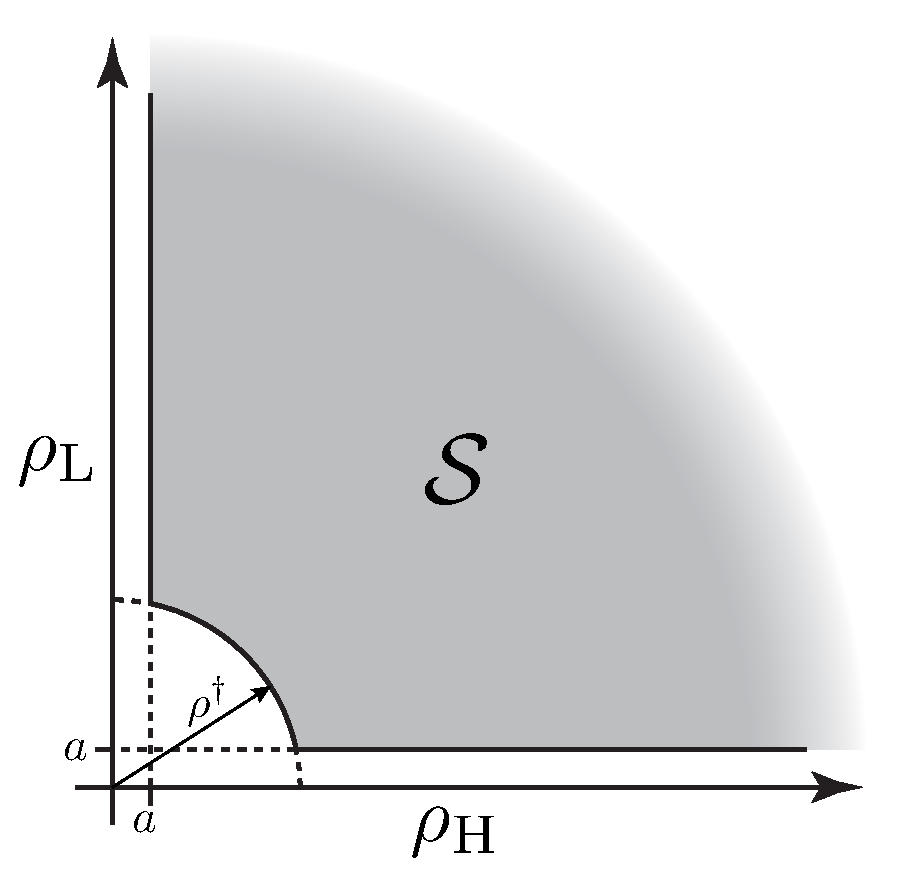
\includegraphics[height=4.25in]{figures/SNRintegrationRegion.pdf} \\
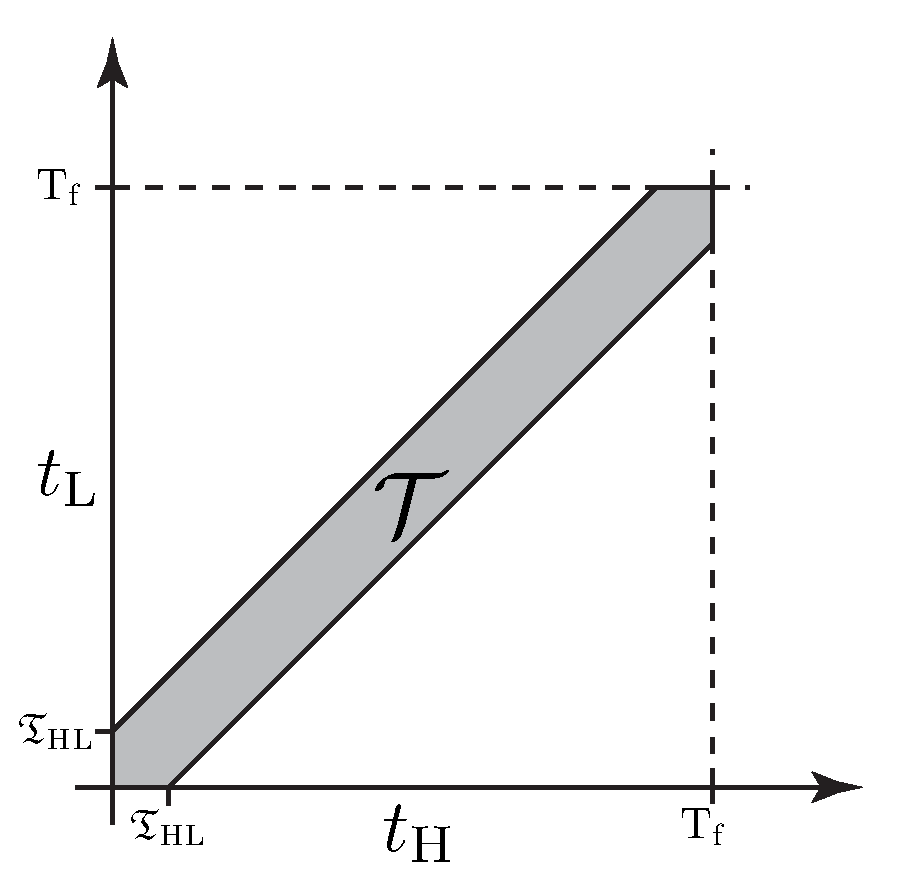
\includegraphics[height=4.25in]{figures/TimeIntegrationRegion.pdf}
\end{center}
\caption{The regions of integration in $\rho$, and time for a network of two detectors, $\varH$ and $\varL$.}
\end{figure}

\section{Computing Background Using Time Slides}
\label{sec:using_time_slides}

The first term in equation \ref{eqn:exampleSources} is the false alarm rate-density that we seek; thus, we could re-write the equation:
\begin{equation}
\tR_{\mathrm{all}}\left(\rho^\dagger \leq \sqrt{\rho_\varH^2 + \rho_\varL^2} \right) = \widetilde{\far}(\rho^\dagger) + \tR_{\mathrm{GW}}\left(\rho^\dagger \leq \sqrt{\rho_\varH^2 + \rho_\varL^2} \right)
\end{equation}
When we do an experiment and perform the coincidence test, we get a measure of $\tR_{\mathrm{all}}$. To get $\widetilde{\far}$ we must separate out the \ac{GW} terms. Unfortunately, we cannot tell the difference between a coincident trigger that came from noise and one that came from a gravitational wave. (If we could, we would not have to do any of this.) Thus, we must find other ways to separate the two. One way to do so is to perform a \emph{time slide}.

Consider what happens if we add a relative time offset to each detector's data-stream that is larger than the coincidence window between them. Doing so causes the gravitational wave triggers to become uncorrelated across the detectors. The rate of coincident noise triggers, however, is unaffected, since they were uncorrelated anyway. Thus, if we perform the same coincidence test on this ``slid" data as we did for the ``zero-lag" data, the expected number of coincidences is (assuming each detector only has one noise source):
\begin{equation}
\label{eqn:exptd_slid_coincs}
\Exptd \left(N_{\mathrm{all}} \left( \rho^{\dagger2} \leq \sum_{i=1}^{N_d}, \Tf, \vec{\mathcal{O}} \right) \right) = \vT(\Tf) \int_{\mathcal{S}} \prod_{i=1}^{N_d} \left( \rsrc_{i,\mathrm{noise}} P_{i,\mathrm{noise}}(\rho_i) + \rsrc_{\mathrm{GW}} P_{i,\mathrm{GW}}(\rho_i) \right) \d \rho_i
\end{equation}
Here we have made the dependence on the time offset explicit by defining an \emph{offset-vector}:

\begin{equation}
\label{eqn:offset_vec}
\vec{\mathcal{O}} = \left[0 ~~ \Delta t_2 ~~ \ldots ~~ \Delta t_{N_d} \right]
\end{equation}
(The offset for one of the detectors is always zero, since we are sliding the detectors with respect to each other.)

For example, in our two-detector case, the expected number of coincidences becomes:
\begin{eqnarray}
\label{eqn:slideTerms}
\lefteqn{ \Exptd\left(N_{\mathrm{all}} \left(\rho^{\dagger2} \leq \rho_\varH^2 + \rho_\varL^2, \Tf, \vec{\mathcal{O}} \right) \right) } \nonumber \\
 & = &  \vT(\mathrm{T_f}) \int_\mathcal{S}  \d \rho_\varH \d \rho_\varL \times \nonumber \\
 & & \left(\rsrc_{\varH,\mathrm{noise}}P_{\varH,\mathrm{noise}}(\rho_\varH) + \rsrc_{\mathrm{GW}}P_{\varH,\mathrm{GW}}(\rho_\varH)\right) \left(\rsrc_{\varL,\mathrm{noise}}P_{\varL,\mathrm{noise}}(\rho_\varL) + \rsrc_{\mathrm{GW}}P_{\varL,\mathrm{GW}}(\rho_\varL)\right) \nonumber \\ 
 & = & \coincT_{\varH\varL}(2\Tf - \coincT_{\varH\varL}) ( \rsrc_{\varH,\mathrm{noise}}\rsrc_{\varL,\mathrm{noise}} ~ \mathcal{I}_{\mathrm{H,noise; L,noise}} + \rsrc_{\varH,\mathrm{noise}}\rsrc_{\mathrm{GW}} ~ \mathcal{I}_{\mathrm{H,noise; L,GW}}  \nonumber \\
 & & ~ + ~ \rsrc_{\mathrm{GW}}\rsrc_{\varL,\mathrm{noise}} ~ \mathcal{I}_{\mathrm{H,GW; L,noise}} + \rsrc_{\mathrm{GW}}^2 ~ \mathcal{I}_{\mathrm{H,GW; L,GW}} ) 
\end{eqnarray}
where:
\begin{eqnarray}
\label{eqn:HnoiseLnoiseIntegral}
\mathcal{I}_{\mathrm{H,noise; L,noise}} & = & \frac{1}{2\pi \sigma_{\varH,\mathrm{noise}} \sigma_{\varL,\mathrm{noise}}} \int_{\mathcal{S}} e^{-(\rho_{\varH}^2 / 2\sigma_{\varH,\mathrm{noise}}^2 + \rho_{\varL}^2 / 2\sigma_{\varL,\mathrm{noise}}^2 )} \d \rho_{\varH} \d \rho_{\varL} \\
\label{eqn:HnoiseLgwIntegral}
\mathcal{I}_{\mathrm{H,noise; L,GW}} & = & \frac{4\pi \sigma_{\mathrm{GW}}^3}{(2.26)^3 \sqrt{2\pi} \sigma_{\varH,\mathrm{noise}}} \int_{\mathcal{S}} \rho_\varL^{-4} e^{-\rho_{\varH}^2 / 2\sigma_{\varH,\mathrm{noise}}^2} \d \rho_\varH \d \rho_\varL \\
\label{eqn:HgwLnoiseIntegral}
\mathcal{I}_{\mathrm{H,GW; L,noise}} & = & \frac{4\pi \sigma_{\mathrm{GW}}^3}{(2.26)^3 \sqrt{2\pi} \sigma_{\varL,\mathrm{noise}}} \int_{\mathcal{S}} \rho_\varH^{-4} e^{-\rho_{\varL}^2 / 2\sigma_{\varL,\mathrm{noise}}^2} \d \rho_\varH \d \rho_\varL \\
\label{eqn:HgwLgwIntegral}
\mathcal{I}_{\mathrm{H,GW; L,GW}} & = & \left( \frac{4\pi \sigma_{\mathrm{GW}}^3}{(2.26)^3} \right)^2 \int_{\mathcal{S}} \rho_\varH^{-4} \rho_\varL^{-4} \d \rho_\varH \d \rho_\varL
\end{eqnarray}
(Of the four, the only integral that can be solved analytically in region $\mathcal{S}$ is the GW/GW term\footnote{Note that if we did not impose the \ac{SNR} cut-off at $a$ then the GW/GW integral would give infinity; i.e., we would expect an infinite number of events in the detector from gravitational waves! This is a result of the model we have chosen for \acp{GW}. If the limits of integration were $\rho = 0,\infty$, then, from equation \ref{eqn:DtoRho}, we would be considering every source from here to infinity. By assuming that the distribution of sources is uniform throughout the universe (which we did by setting $\rsrc_{\mathrm{GW}}(\vec{\theta})$ to a constant), this means that if we look for an infinite distance, we will get an infinite number of sources --- a \ac{GW} version of Oblier's paradox \cite{obliers_paradox}. Of course, the real universe is not infinitely old; beyond $\sim 1\,\mathrm{Gpc}$ the number of \acp{CBC} begins to fall off \cite{rates_paper}. Further, we have assumed that the GW/GW term is independent of the noise. In practice, however, we do clustering, which couples these terms. Even if we had an ideal detector with stationary Gaussian noise in \ac{SNR}, below some \ac{SNR} the noise triggers would effectively cluster away all \ac{GW} events, even if the universe was infinitely old. We get around both of these difficulties by assuming that the \ac{SNR} cutoff is high enough that these effects do not affect our model (which, with $a=5.5$, is valid for both enhanced and advanced \ac{LIGO}.}, which is:
\begin{eqnarray}
\lefteqn{ \mathcal{I}_{\mathrm{H,GW;L,GW}} = } \nonumber \\
 & & \left( \frac{4\pi \sigma_{\mathrm{GW}}^3}{(2.26)^3} \right)^2 \left( \frac{\rho^{\dagger2} - 2a^2}{18 \rho^{\dagger6} a \sqrt{\rho^{\dagger2} - a^2}} \left( 1 + \frac{\rho^{\dagger4}}{8a^2\left(\rho^{\dagger2} - a^2 \right)} \right) + \frac{1}{9a^3 \left(\rho^{\dagger2} - a^2 \right)^{3/2}} \right)
\end{eqnarray}
if $\rho^\dagger \geq \sqrt{2}a$;
\begin{equation}
\mathcal{I}_{\mathrm{H,GW;L,GW}} = \left( \frac{4\pi \sigma_{\mathrm{GW}}^3}{(2.26)^3} \right)^2 \frac{1}{9a^6}
\end{equation}
otherwise. The other three integrals can be solved numerically, however; see Chapter \ref{ch:future_developments} for details.)

By de-coupling the gravitational waves in each detector, the GW/GW term is now much smaller than in the zero-lag case. For example, we can calculate the expected number of GW/GW coincidences for a $1.4/1.4\,\Msun$ binary neutron star system in each case. From \cite{rates paper}, the rate of \ac{BNS} coalescences in the universe is $\rsrc_{\mathrm{GW}} = 1 \times 10^{-6} \Mpc^{-3}\,\mathrm{yr}^{-1}$. During enhanced \ac{LIGO}, the $4\,\mathrm{km}$ \ac{LIGO} interferometers had a peak horizon distance to \ac{BNS} systems of $\sim40\Mpc$, which gives a sensitivity of $\sigma_{\mathrm{GW}} = \rho D_{\mathrm{horizon}} = 8 \times 40\Mpc = 320\Mpc$. Thus, if our two hypothetical detectors had the same sensitivity, then in one year we would expect:

\begin{eqnarray}
\Exptd\left( N_{\mathrm{GW}} \left( \rho^{\dagger}  =  11.3, \Tf = 1 \,\mathrm{yr} \right)\right) & = & \frac{4}{3} \pi \frac{\sqrt{2} (320\Mpc)^3}{(2.26)^3 (11.3 / \sqrt{2})^3} (1 \times 10^{-6}\Mpc^{-3}\,\mathrm{yr^{-1}}) (1\,\mathrm{yr}) \nonumber \\
 & = & 0.03 \nonumber
\end{eqnarray}
gravitational-wave events in zero-lag at a New \ac{SNR} of $8$ in each detector (which corresponds to a combined New SNR of $\rho^\dagger = \sqrt{2} \times 8 = 11.3$). In contrast, the expected number of coincident gravitational-waves in a one year-long time slide would be:

\begin{eqnarray}
\lefteqn{\Exptd\left( N_{\mathrm{GW}} \left(\rho^{\dagger} = 11.3, \Tf = 1\,\mathrm{yr}, \mathcal{O} \right) \right) } \nonumber \\
& = & (3.2 \times 10^{-10}\yr) ( 2\yr - 3.2\times10^{-10}\yr ) (1\times10^{-6}\Mpc^{-3}\yr^{-1})^2 \mathcal{I}_{\mathrm{H,GW;L,GW}}(\rho^\dagger = 11.3, a = 5.5) \nonumber \\
& = & 6 \times 10^{-13} \nonumber
\end{eqnarray}
Here, we have a coincidence window of $\coincT_{\varH\varL} = 10\,\mathrm{ms} \approx 3.2\times10^{-10}\yr$. This is about the light-travel time between Hanford and Livingston.

As can be seen in equation \ref{eqn:slideTerms}, doing the time slide has introduced mixing terms between \acs{GW} and noise. However, evaluating the integrals \ref{eqn:HnoiseLnoiseIntegral}--\ref{eqn:HgwLnoiseIntegral} requires fitting to data in order to determine $\sigma_{i,\mathrm{noise}}$ and $\rsrc_{i,\mathrm{noise}}$. Here we will assume the noise/GW terms are small relative to the noise/noise term, using the fact that number of expected gravitational waves in enhanced \ac{LIGO} is less than one as our reasoning. For a further discussion of the effect of these mixing terms, see Chapter \ref{ch:future_developments}.

Since the noise/noise term is the dominate source in a time-slide, we have:
\begin{equation}
\label{eqn:valid_slide_condition}
\tR_{\mathrm{all}}\left(\rho^{\dagger2} \leq \sum_{i=1}^{N_d} \rho_i^2, \mathcal{O} \right) \approx \widetilde{\far}(\rho^\dagger)
\end{equation}
Thus, we can measure the false alarm rate of a trigger with combined New \ac{SNR} $\rho^\dagger$ by simply performing a time slide, counting the number of coincidences that have a combined New \ac{SNR} $\geq \rho^\dagger$, and dividing by the slide duration. This method has the further advantage that we can perform multiple slides with the same data to improve our measurement of $\widetilde{\far}$. If we change the offset of each detector by enough to consider every slide to be independent --- i.e., we slide the data enough so that no two events can be coincident in more than one slide ---  then, from equation \ref{eqn:avg_rate_param}, in $N_t$ slides:

\begin{equation}
\label{eqn:meanFAR1}
\overline{\far}(\rho^\dagger) = \frac{\sum_{k=1}^{N_t} \widehat{N}_k \left(\rho^{\dagger2} \leq \sum_{i=1}^{N_d} \rho_i^2 \right)}{\Tb} 
\end{equation}
where $\widehat{N}_k \left(\rho^{\dagger2} \leq \sum_{i=1}^{N_d} \rho_i^2 \right)$ is the measured number of coincidences with a combined New \ac{SNR} $\geq \rho^\dagger$ in the $k\th$ slide, and $\Tb$ is the total \emph{background time}. The background time is the sum of the length of each slide; the length of each slide is the intersection of every detector's foreground analysis time after they have been slid. Therefore:

\begin{equation}
\label{eqn:tBackground}
\Tb = \sum_{k=1}^{N_t} \left| \left( \mathbb{T}^A + \mathcal{O}_k[A] \right) \bigcap \left( \mathbb{T}^B + \mathcal{O}_k[B] \right) \bigcap \ldots \bigcap \left( \mathbb{T}^{N_d} + \mathcal{O}_k[N_d] \right) \right|
\end{equation}
(Here, $\mathbb{T}^i$ is the analysis segment of the $i\th$ detector; $\left| \mathbb{T}^i \right| = \Tf^i$.) With a finite data set, a single \emph{linear} slide will not have the same duration as the foreground time since the overlap between detectors will decrease with increasing offsets. If the slide is done on a \emph{ring}, so that data that is slid past the end of the segment is put at the beginning, than a slide will have the same duration as the zero-lag. However, if there are gaps in the data, then even sliding on a ring will result in different durations from slide-to-slide, since the gaps will align differently in each slide. We therefore define the \emph{effective number of slides}, $\widetilde{N}_t$, as the ratio of the total background time to the foreground time:
\begin{equation}
\label{eqn:effective_Nslides}
\widetilde{N}_t \equiv \frac{\Tb}{\Tf}
\end{equation}
so that equation \ref{eqn:meanFAR1} can be written:
\begin{equation}
\label{eqn:meanFAR2}
\overline{\far}(\rho^\dagger) = \frac{\widehat{N}_{\mathrm{total}} \left(\rho^{\dagger2} \leq \sum_{i} \rho_i^2 \right)}{\Tf \widetilde{N}_t} = \frac{\overline{N} \left(\rho^{\dagger2} \leq \sum_{i} \rho_i^2 \right)}{\Tf}
\end{equation}
Since the sum over the number of slides in the numerator of equation \ref{eqn:meanFAR1} is simply a sum of counts, here we have written it as $\widehat{N}_{\mathrm{total}} \left(\rho^{\dagger2} \leq \sum_{i} \rho_i^2 \right)$, which is the total number of triggers with combined New \ac{SNR} $\geq \rho^\dagger$ (\emph{false alarms}) in all the slides. Thus, $\overline{N} \left(\rho^{\dagger2} \leq \sum_{i} \rho_i^2 \right)$ is the average number of false alarms in a single experiment with a duration equal to $\Tf$. Since this is the mean of a stationary Poisson process, from equation \ref{eqn:err_R}, the error in $\overline{\far}$ is:
\begin{eqnarray}
\label{eqn:err_FAR}
\delta \overline{\far}(\rho^\dagger) & = & \frac{1}{\Tf} \sqrt{\frac{\overline{N} \left(\rho^{\dagger2} \leq \sum_{i} \rho_i^2 \right)}{\widetilde{N}_t}} \nonumber \\
 & = & \frac{1}{\Tf} \sqrt{\frac{\widehat{N}_{\mathrm{total}} \left(\rho^{\dagger2} \leq \sum_{i} \rho_i^2 \right)}{\widetilde{N}_t^2}} \nonumber \\
 & = & \frac{\sqrt{\widehat{N}_{\mathrm{total}} \left(\rho^{\dagger2} \leq \sum_{i} \rho_i^2 \right)}}{\Tb}
\end{eqnarray}

We have arrived at a way to calculate false alarm rates for a single template: perform the coincidence test in several times slides; compute the duration of each time slide; count the number of slide coincidences in all slides that have a combined New \ac{SNR} greater-than-or-equal to a given foreground New \ac{SNR}; divide by the total background time.

\section{Computing FARs with Multiple Templates}
\label{sec:mulitple_templates}

To compute a false alarm rate across a bank of templates, we would replace the time integral in equation \ref{eqn:N_general_prob} with an integral over the template parameters, $\{\vartheta_m\}$, bounded by the ethinca ellipsoid at $\rho$, $\mathcal{E}(\rho)$:

\begin{equation}
\Exptd\left(N_{\mathrm{uncorr}}\left(\rho^{\dagger2} \leq \sum_i\rho_i^2, \Tf \right)\right) = \int_{\mathcal{S}(\rho^\dagger)} \int_{\mathcal{E(\rho)}} \prod_i^{N_d} \sum_j^{N_s}  \prod_{m}^{n_p} \rsrc_{i,j} P_{i,j}(\rho_i, \{\vartheta_m \}) \d \vartheta_m \d t_i \d \rho_i
\end{equation}
where $n_p$ is the number of parameters used. For example, in a non-spinning search in which the templates are laid out in $\tau_0$ and $\tau_3$ space, this would be:
\begin{equation}
\Exptd\left(N_{\mathrm{uncorr}}\left(\rho^{\dagger2} \leq \sum_i\rho_i^2, \Tf \right)\right) = \int_{\mathcal{S}(\rho^\dagger)} \int_{\mathcal{E(\rho)}} \prod_i^{N_d} \sum_j^{N_s}  \rsrc_{i,j} P_{i,j}(\rho_i, \tau_0, \tau_3) \d \tau_0 \d \tau_3 \d t_i \d \rho_i
\end{equation}

Ideally, the probability of getting a trigger would be independent of the template parameters. In that case, the integral over $\mathcal{E}(\rho)$ could be carried out independent of the source \acp{PDF}, as was done with the time integral in section \ref{sec:coincidence_modelling}. This would mean that the number of coincident triggers with a combined New \ac{SNR} $\geq$ to any given value would only be dependent on $\rho$. This is ideal, since the false alarm rate is meant to be a measure of how likely a trigger is a gravitational wave, independent of parameters. It would also mean that we could simply count the number of slide coincidences to get the false alarm rate, as described above, without needing any correction for the parameters of the templates.

In practice, however, the false alarm rate of a template \emph{is} dependent on its parameters. Figure \ref{fig:newsnr_v_mchirp} shows the dependence of the cumulative rate of coincident slide triggers on chirp mass ($\mathcal{M}$) when the rates are based on New \ac{SNR}. These triggers were taken from $100$ slides in six weeks (about $0.03\,\mathrm{yr}$ of analysis time) of enhanced \ac{LIGO} data in which the $4\,\mathrm{km}$ Hanford (H1) and Livingston (L1) detectors were analyzed (``S6"; see Chapter \ref{ch:s6_results} for details). As can be seen in Figure \ref{fig:newsnr_v_mchirp-a}, the overall rate of triggers decreases with increasing chirp mass. This is due to the fact that the template bank is more sparsely populated at higher masses. Conversely, the variance of the rate of triggers roughly increases with increasing mass, leading to a higher rate of high New \ac{SNR} triggers at high mass. This occurs because the inspiral phase of a higher-mass template spends less time in band compared to lower masses. As a result, $\chi^2$ does a poorer job distinguishing high mass \acp{CBC} from glitches, which also tend to ring off the higher masses with larger \ac{SNR}.

The joint effect of the lower overall rate and higher variance of high-mass templates can be seen in Figure \ref{fig:newsnr_v_mchirp-b}, which plots the combined New \ac{SNR} of the triggers versus chirp mass. (To go from \ref{fig:newsnr_v_mchirp-a} to \ref{fig:newsnr_v_mchirp-b}, think of the color bar as the z-axis, and imagine rotating the axes so that $x \rightarrow y$, $y \rightarrow z$, and $z \rightarrow x$.) Due to the decrease in the overall rate, the cumulative rate drops off with increasing chirp mass at low combined New \ac{SNR} (orange -- yellow lines in the figure). However, due to the higher variance, the rate increases with increasing chirp mass (up to the middle of the chirp-mass space, anyhow) at large combined New \ac{SNR} (the red line in the figure). This latter effect can be particularly problematic since we are most interested in triggers with higher New \ac{SNR}. For example, consider what were to happen if a binary neutron star template with $\mathcal{M} = 2\,\Msun$ rang off with a New \ac{SNR} of 10.5. If our template bank was restricted to binary neutron stars ($\mathcal{M} \approx 1$--$3\,\Msun$), the trigger would stick well above background, as can be seen in Figure \ref{fig:newsnr_v_mchirp-b}. However, if we include the entire bank in the false alarm calculation, then the event would be out-ranked by the two events between $\mathcal{M} = 7$--$9\,\Msun$, leading to a $\far \approx 50\,\mathrm{yr}^{-1}$. This high \ac{FAR} would have more to do with our ranking statistic's inability to take into account the parameters of the template than with our degree of belief in how likely the trigger is a gravitational wave.

One way to fix this is to break up the chirp-mass space when computing \acp{FAR}. If we bin the space such that the cumulative rate is roughly constant for a given New \ac{SNR} across the bin, then we can use our naive approach of counting slide triggers to get $\far$. The $\far$ computed in each bin, however, is not the true \ac{FAR} for the search, since we sliced up the parameter space in order to arrive at it. To understand why the slicing needs to be accounted for, consider the number of bins. Our initial choice of bins was arbitrary: we could choose to slice the parameter space up even more; in so doing, we would get a smaller $\far$. Yet this plummeting \ac{FAR} would have little to do with the likelihood that the triggers are gravitational waves and everything to do with our choice of bins. Thus, to fix this, we must compute a \emph{combined \ac{FAR}}, $\cfar$, across all of the bins.

In order to compute a combined \ac{FAR}, we use the \emph{uncombined} \ac{FAR} --- i.e., the \acp{FAR} computed using the bins --- as our ranking statistic. This means we must compute an uncombined \ac{FAR} for the slide triggers. We do this in the same manner that we compute uncombined \acp{FAR} for zero-lag triggers: we count the number of slide triggers that have a combined New \ac{SNR} $\geq$ the $\rho$ of a given trigger. By doing so we treat a given slide as if it were zero-lag. Thus, we do not include the slide in which we are computing uncombined \acp{FAR} in the background estimate for that slide. Since we use one-less slide for measurement of the background triggers' \acp{FAR}, the error in our measurement of the slide triggers \acp{FAR} will be larger than that of zero-lag triggers. Assuming each slide has roughly the same duration then, from equation \ref{eqn:err_FAR}, the error is increased to:

\begin{equation}
\label{eqn:err_FAR_slide}
\delta \overline{\far}_{\mathrm{slide}} \approx \frac{\sqrt{ \widehat{N}_{\mathrm{total}} ( 1 - \widetilde{N}_t^{-1} ) }}{ \Tb (1- \widetilde{N}_t^{-1}) }
\end{equation}
For large $N_t$, however, the discrepancy between the zero-lag and time-slide $\delta \far$ is small. 

Once we have uncombined \acp{FAR} for both foreground and background triggers, we compute the combined \acp{FAR} by counting the total number of triggers with a $\far$ \emph{less-than} the given trigger's \ac{FAR}, $\far^\dagger$:

\begin{equation}
\label{eqn:cfar_1}
\overline{\cfar}( \far^\dagger ) = \frac{ \widehat{N}_{\mathrm{total}}\left( \far < \far^\dagger \right) }{\Tb}
\end{equation}
The reason we count the number of triggers that have a \ac{FAR} \emph{less-than} and not \emph{less-than or equal-to} $\far^\dagger$ can be understood by considering what happens to a trigger that has a $\rho$ larger than all the background in its bin. If a trigger is louder than all the background, it will have a measured \ac{FAR} of 0. This does not mean we are absolutely certain the trigger is a gravitational wave. A \ac{FAR} of 0 means that we have set an upper-limit on the true \ac{FAR} to be less-than $1/\Tb$, within the error bars; i.e.:

\begin{equation}
\label{eqn:zeroFAR}
\overline{\far}(\rho^\dagger) = 0 \Rightarrow \widetilde{\far}(\rho^\dagger) < \frac{1}{\Tb} \pm \frac{1}{\Tb}
\end{equation}
Since we have only placed an upper limit on the uncombined \ac{FAR}, we should also only be able to place a limit on the combined \ac{FAR}; thus, if we got zero for $\far^\dagger$ we should also get zero for $\cfar^\dagger$. (The combined \ac{FAR} limit will be higher however; specifically, it will be $N_{\mathrm{bins}}/\Tb$, where $N_{\mathrm{bins}}$ is the number of bins.) Yet if we have, say, $N_0$ triggers in the background with $\far = 0$ and we were to count the number of triggers $\leq \far^\dagger$, we would get a combined \ac{FAR} \emph{equal} to $N_0/\Tb$, not less-than. Thus, we would have extracted a measured value for the combined \ac{FAR} from a limit, without having had any new information about the trigger.

Breaking up the parameter space into bins and computing combined \acp{FAR} from uncombined allows us to map the triggers onto a space where the parameter dependence has been removed. Note, however, that since a slide is not counted against itself, in each bin we will have at least one trigger with $\overline{\far} = 0$. This is the trigger that has the largest value of $\rho$; i.e., it is the loudest background trigger. (We could have more than one slide trigger in a bin with $\overline{\far} = 0$ if a single slide contained multiple triggers that were louder than the triggers in all other slides.) Thus, if we have $N_{\mathrm{bins}}$ bins, we will have at least $N_{\mathrm{bins}}$ background triggers with $\overline{\far} = 0$. This means that if a foreground trigger has $\overline{\far} = 1/\Tb$ in its bin, it will have $\overline{\cfar} = N_{\mathrm{bins}}/\Tb$. In other words, even if a foreground trigger has a $\rho$ that is far larger than all but one slide trigger, and that slide trigger is in the same bin, its combined \ac{FAR} will increase by at least a factor of $N_{\mathrm{bins}}$. If a trigger has a zero uncombined \ac{FAR} (and therefore a zero combined \ac{FAR}), the smallest upper limit that can be placed on its true false alarm rate will also increase according to the number of bins, or \emph{trials factors}. The number of bins should therefore be kept to a minimum.

Figure \ref{fig:ufar_v_mchirp} shows the background distribution in uncombined \ac{FAR} of the same set of triggers used in Figure \ref{fig:newsnr_v_mchirp}. The bins used are clearly visible via the ``steps" in Figure \ref{fig:ufar_v_mchirp-b}. These bins --- which are $\mathcal{M}/\Msun \in \{ [0.0, 3.48); [3.48, 7.4); [7.4,\infty) \}$ --- are the same that were used in the analysis of LIGO's fifth and sixth science runs (S5 and S6, respectively). As can be seen by the lines of constant high cumulative rate in Figure \ref{fig:ufar_v_mchirp-b} (orange -- yellow lines), the bins are not sufficient to make the rate completely independent of the mass. Indeed, this is impossible with any choice of bins, since there are simply not enough triggers at high mass to extend the high cumulative rate lines into that region. However, for \emph{low} cumulative rates, the space has been sufficiently ``flattened." Note, in particular, the red line, which shows a cumulative rate of $1/\Tb$ in each bin. In Figure \ref{fig:newsnr_v_mchirp-b}, this line dropped off at low chirp mass, which would cause low-mass systems to get higher-than-expected false alarm rates, as in the case of the \ac{BNS} system above. Now, low-mass systems with high $\rho$ are ranked on par with the medium mass systems. Since these are the triggers we are most interested in, this choice of bins is sufficient for our purposes, and we have only incurred a trials factor of 3.

There is one last parameter that we need to be aware of when choosing the number of bins: the number of detectors contributing to the coincidence. Since combined New \ac{SNR} is computed by taking the quadrature sum of the single-\ac{IFO} New \acp{SNR}, coincidences that have a larger number of contributing detectors will have a larger combined $\rho$. For example, if we analyze three detectors --- call them H, L, and V --- then we can have four types of coincidences: HL, HV, LV, and HLV. A trigger with New \ac{SNR} $= 8$ in each detector will have a combined New \ac{SNR} $= \sqrt{2}\times8$ if it is a HL, HV, or LV coincidence, and a combined New \ac{SNR} $= \sqrt{3}\times8$ if it is a triple coincidence. That may seem appropriate: after all, the more detectors that observe the event, the more likely we are to believe it to be a \ac{GW}. However, due to the antenna pattern of the detectors, and the fact that they are not co-located nor have the same sensitivity, a \ac{GW} will not be seen in all detectors if it came from a source in certain sky locations and orientations. If we were to compute \acp{FAR} without first binning the triggers by the number of coincident triggers, or \emph{coincidence type}, we would subtly introduce a location and orientation bias into the \ac{FAR}. To avoid this, we also bin triggers by their coincidence type.\footnote{Admittedly, simply binning the triggers by coincidence type then using the uncombined \acp{FAR} to get the combined \ac{FAR} is not the perfect solution to remove biases either. Doing so treats all the coincidence types with equal weight. However, if the detectors have varying sensitivities, it is more likely to get a gravitational wave from coincidences of the most sensitive detectors. A better approach would be to add some weight to each coincidence type that is proportional to the sensitivity of the constituent detectors before combining the \acp{FAR}. The same argument applies to mass-bins: if the detectors are more sensitive to certain parameter ranges, we should weight accordingly. A likelihood-based weighting that attempted to remedy these concerns was used in the joint LIGO-Virgo search in the last few months of \ac{S5}; see \cite{ref:LVC_paper} for details. For the rest of \ac{S5} and \ac{S6}, the detectors' sensitivities were roughly on-par with each other, so the simpler equal-weight method described here was used.}

Across the course of an analysis period varying combinations of detectors will be available to analyze. (An \ac{IFO} is not analyzable if it is not in \emph{Science} mode, which can occur if it ``loses lock"; see Chapter \ref{ch:ihope_pipeline} for details.) For example, in the three detector case given above, we can have four different \emph{instrument times}: periods when HLV were on, and periods when HL, HV, or LV were on. Obviously, only certain coincident types can occur in a given period. Therefore, when computing a \ac{FAR} for a trigger, we should not include analysis times in which it was impossible for the coincidence type of the trigger to occur. If we did, we would artificially decrease the false alarm rate of the trigger. As a result, each of the various instrument times are treated as independent experiments: both uncombined and combined \acp{FAR} are computed within the instrument time, and \acp{FAR} are never calculated across instrument times. This also means that coincidences of the same type cannot be combined across instrument times. For example, in the three detector case, we can get HL, HV, and LV coincident triggers in both HLV time and each of the respective double-coincident times. However, there is a slight difference between the doubles in triple time and the doubles in double time. The double-coincident triggers in HLV time are triggers that were coincident with one other detector \emph{and not} coincident with the third detector. The doubles in double time, however, consist of triggers that would not have been coincident with the third detector \emph{and} triggers that would have been coincident, had the third detector been on. This latter set is clearly a larger population. Thus, if coincidence types were grouped across instrument times (using the sum of the instrument times for the analysis time), we would underestimate the \acp{FAR} of the triggers from double-time and overestimate the \acp{FAR} from triple-time.\footnote{We can, however, group coincidence-types together across instrument times if we reanalyze the data with the other detector removed, or \emph{vetoed}. For example, we can group HL triggers in HL time with HL triggers in HLV time if we re-analyzed the HLV data with V removed. This has been done occasionally in order to get a better estimate of double coincident triggers with low or zero \acp{FAR}.} 

Summarizing, the number of bins, or trials factors, that we use depends on how strongly the ranking statistic couples to a parameter and on the number of coincident types possible in the instrument time being analyzed. In the low-mass \ac{CBC} search we use three mass bins based on chirp mass. This means that we have a trials factor equal to $3$ during double-coincident instrument times. During triple-coincident instrument times in which all coincident types are used, this factor increases to 12 ($3$ mass-bins times $4$ possible coincidence types).

\begin{figure}[p]
\begin{center}
\subfigure[Cumulative Rate v. Combined New SNR. Each line represents the cumulative rate in one chirp-mass bin as a function of Combined New SNR, the boundaries of which are shown in (b).]{\label{fig:newsnr_v_mchirp-a}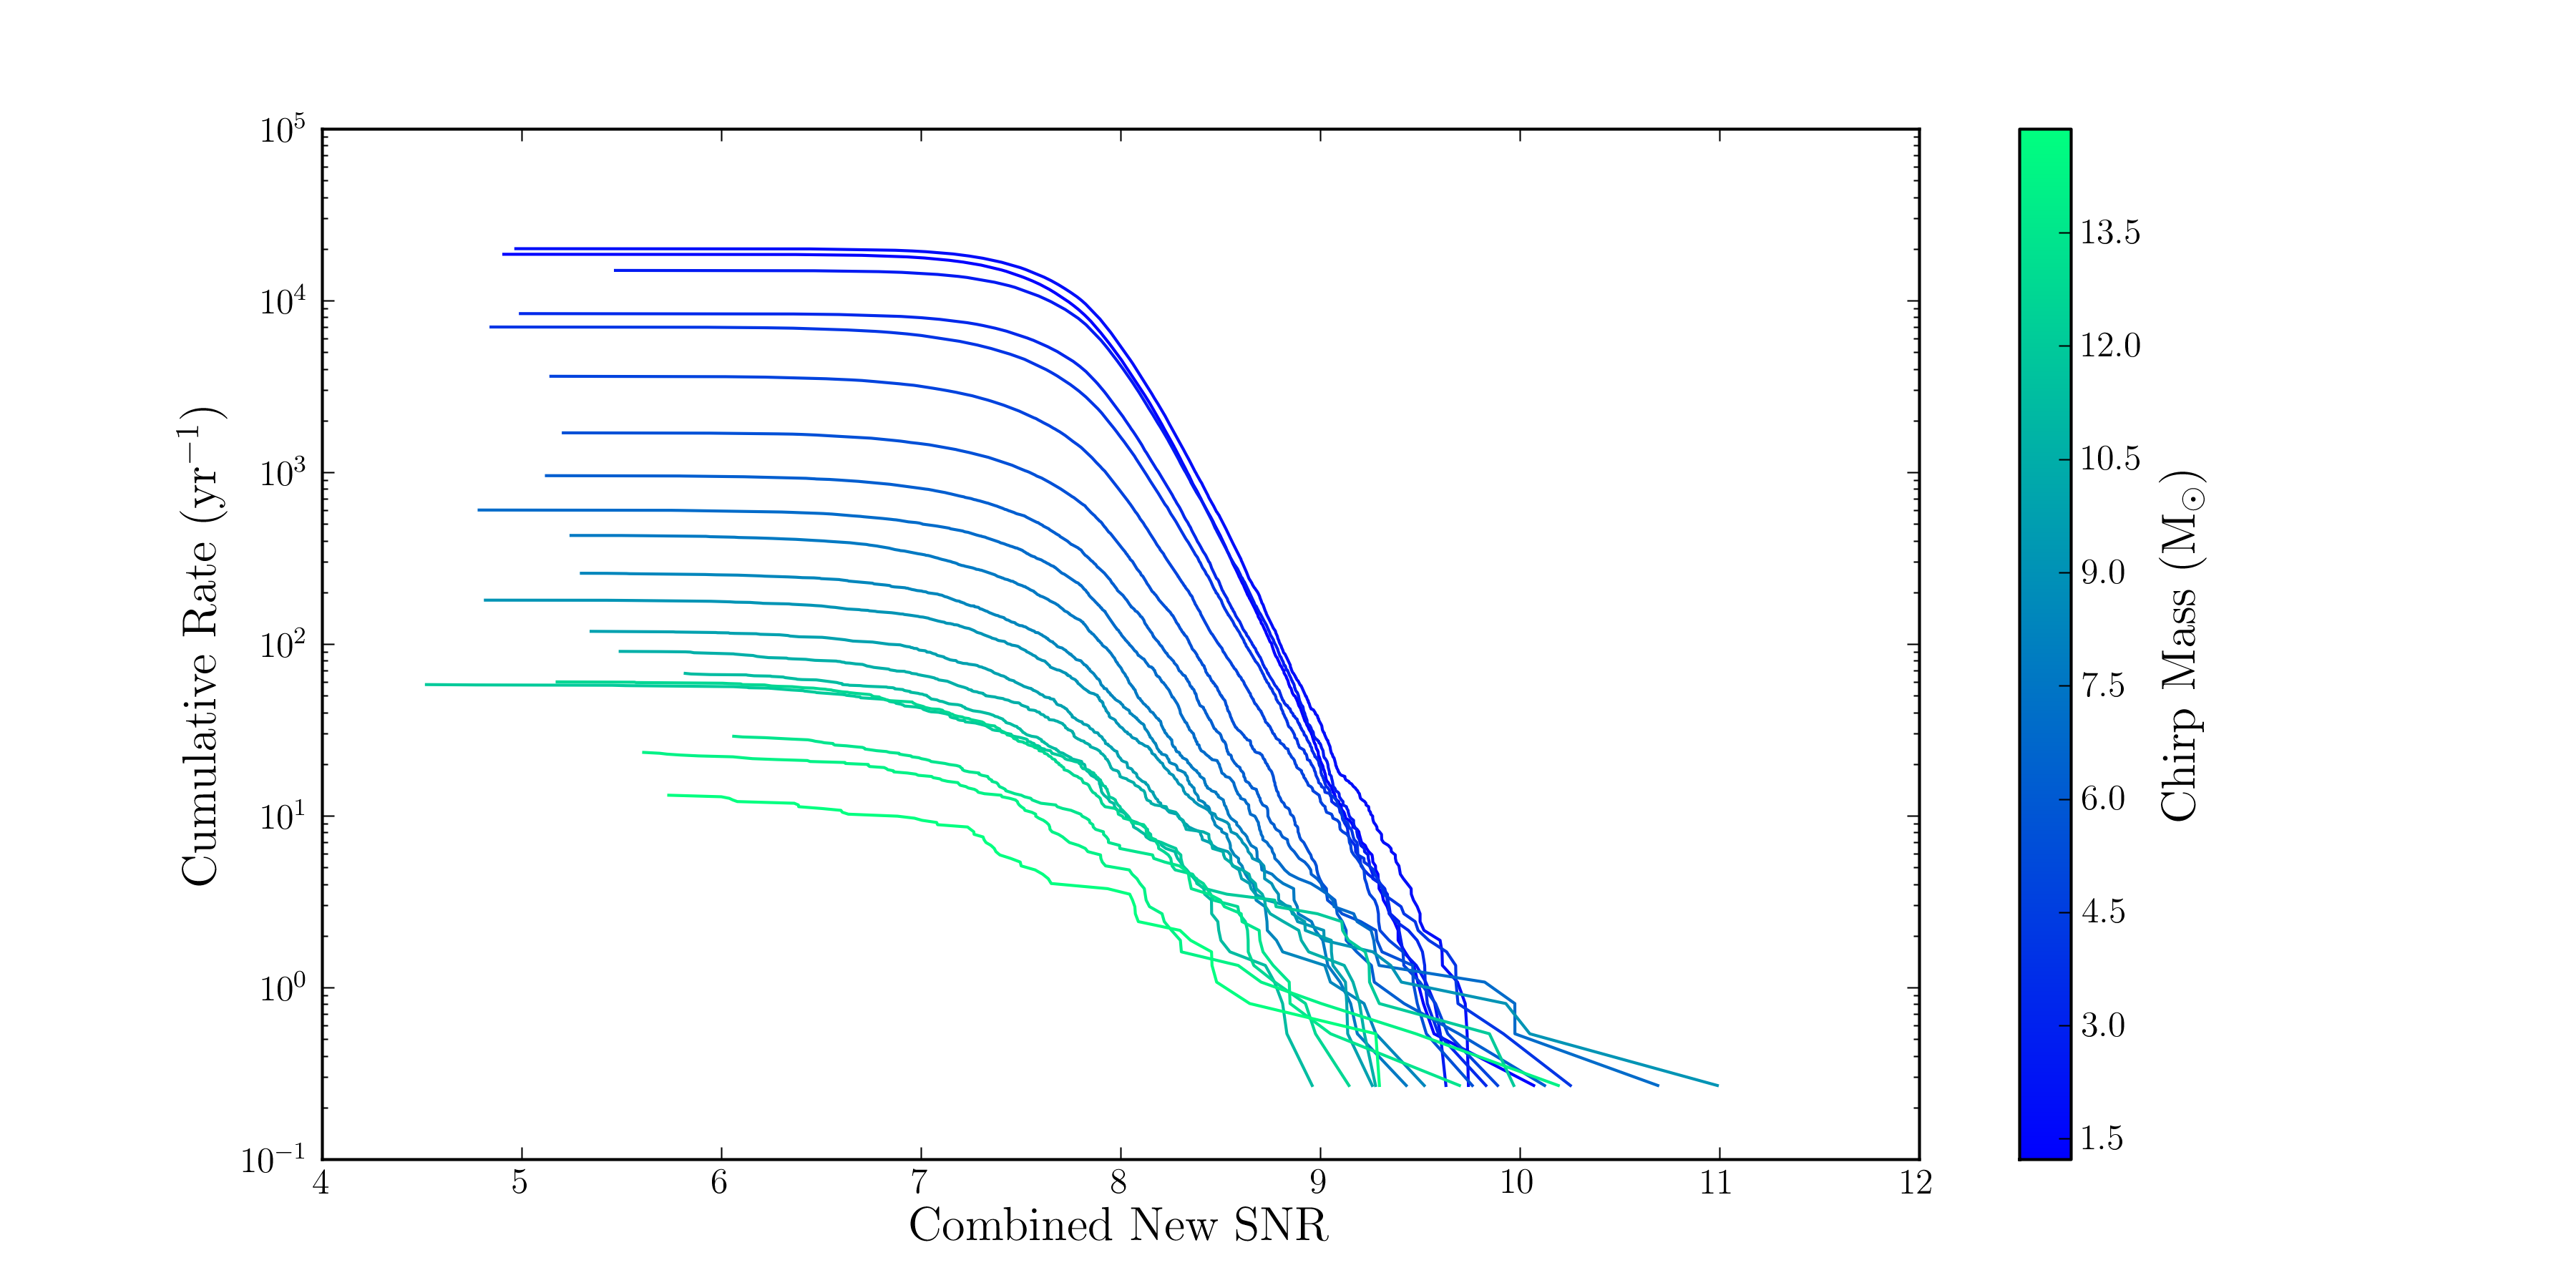
\includegraphics[width=6.5in]{figures/H1L1_H1L1-plotNdensity_cumnum_snr_vs_mchirp.png}}
\subfigure[New SNR v. Chirp Mass. Colored lines show lines of constant cumulative rates across the chirp-mass bins. Dashed lines show the bin boundaries used.]{\label{fig:newsnr_v_mchirp-b}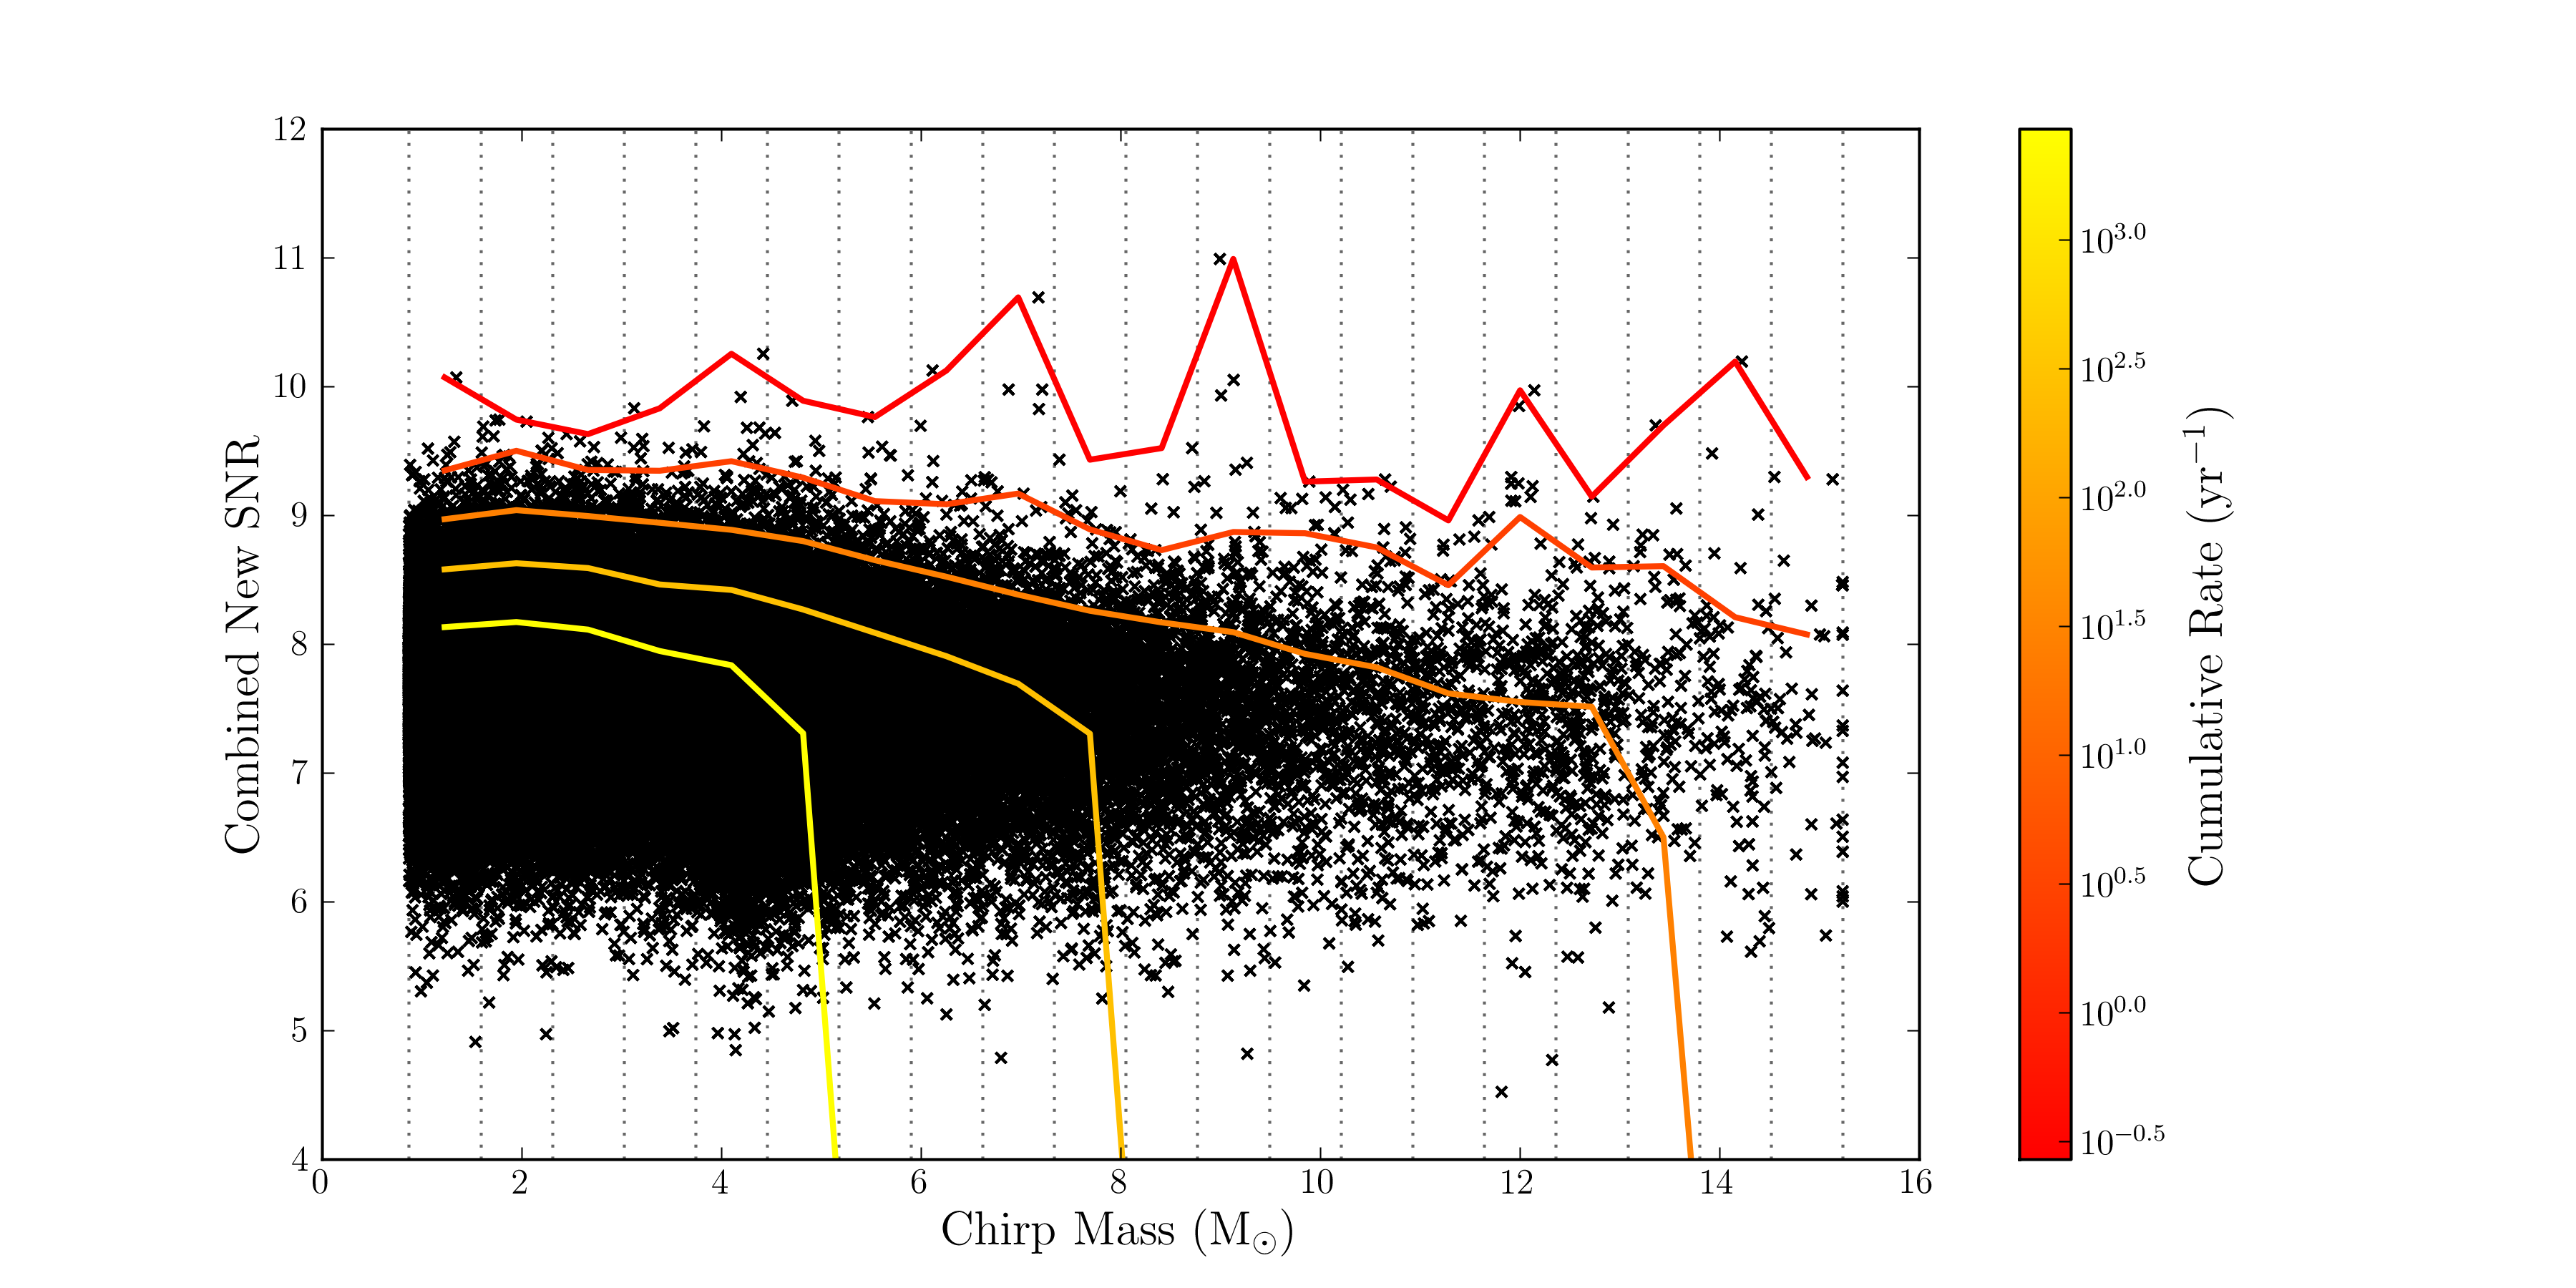
\includegraphics[width=6.5in]{figures/H1L1_H1L1-plotNdensity_snr_vs_mchirp.png}} \\
\end{center}
\caption{The rates of slide coincidences in equally-spaced chirp-mass bins as a function of Combined New SNR. Black crosses are coincident triggers taken from 100 slides in six weeks of enhanced \ac{LIGO} data. The cumulative rates (the y-axis in (a) and the color axis in (b)) are computed by counting the number of triggers with a Combined New SNR $\geq$ each trigger within each bin. Only the $4\,\mathrm{km}$ Hanford (H1) and Livingston (L1) triggers were analyzed during this time; as such, all coincidences are H1L1 triggers.}
\label{fig:newsnr_v_mchirp}
\end{figure}

\begin{figure}[p]
\begin{center}
\subfigure[Cumulative Rate v. Uncombined FAR. Each line represents the cumulative rate in one chirp-mass bin as a function of Uncombined FAR, the boundaries of which are shown in (b).]{\label{fig:ufar_v_mchirp-a}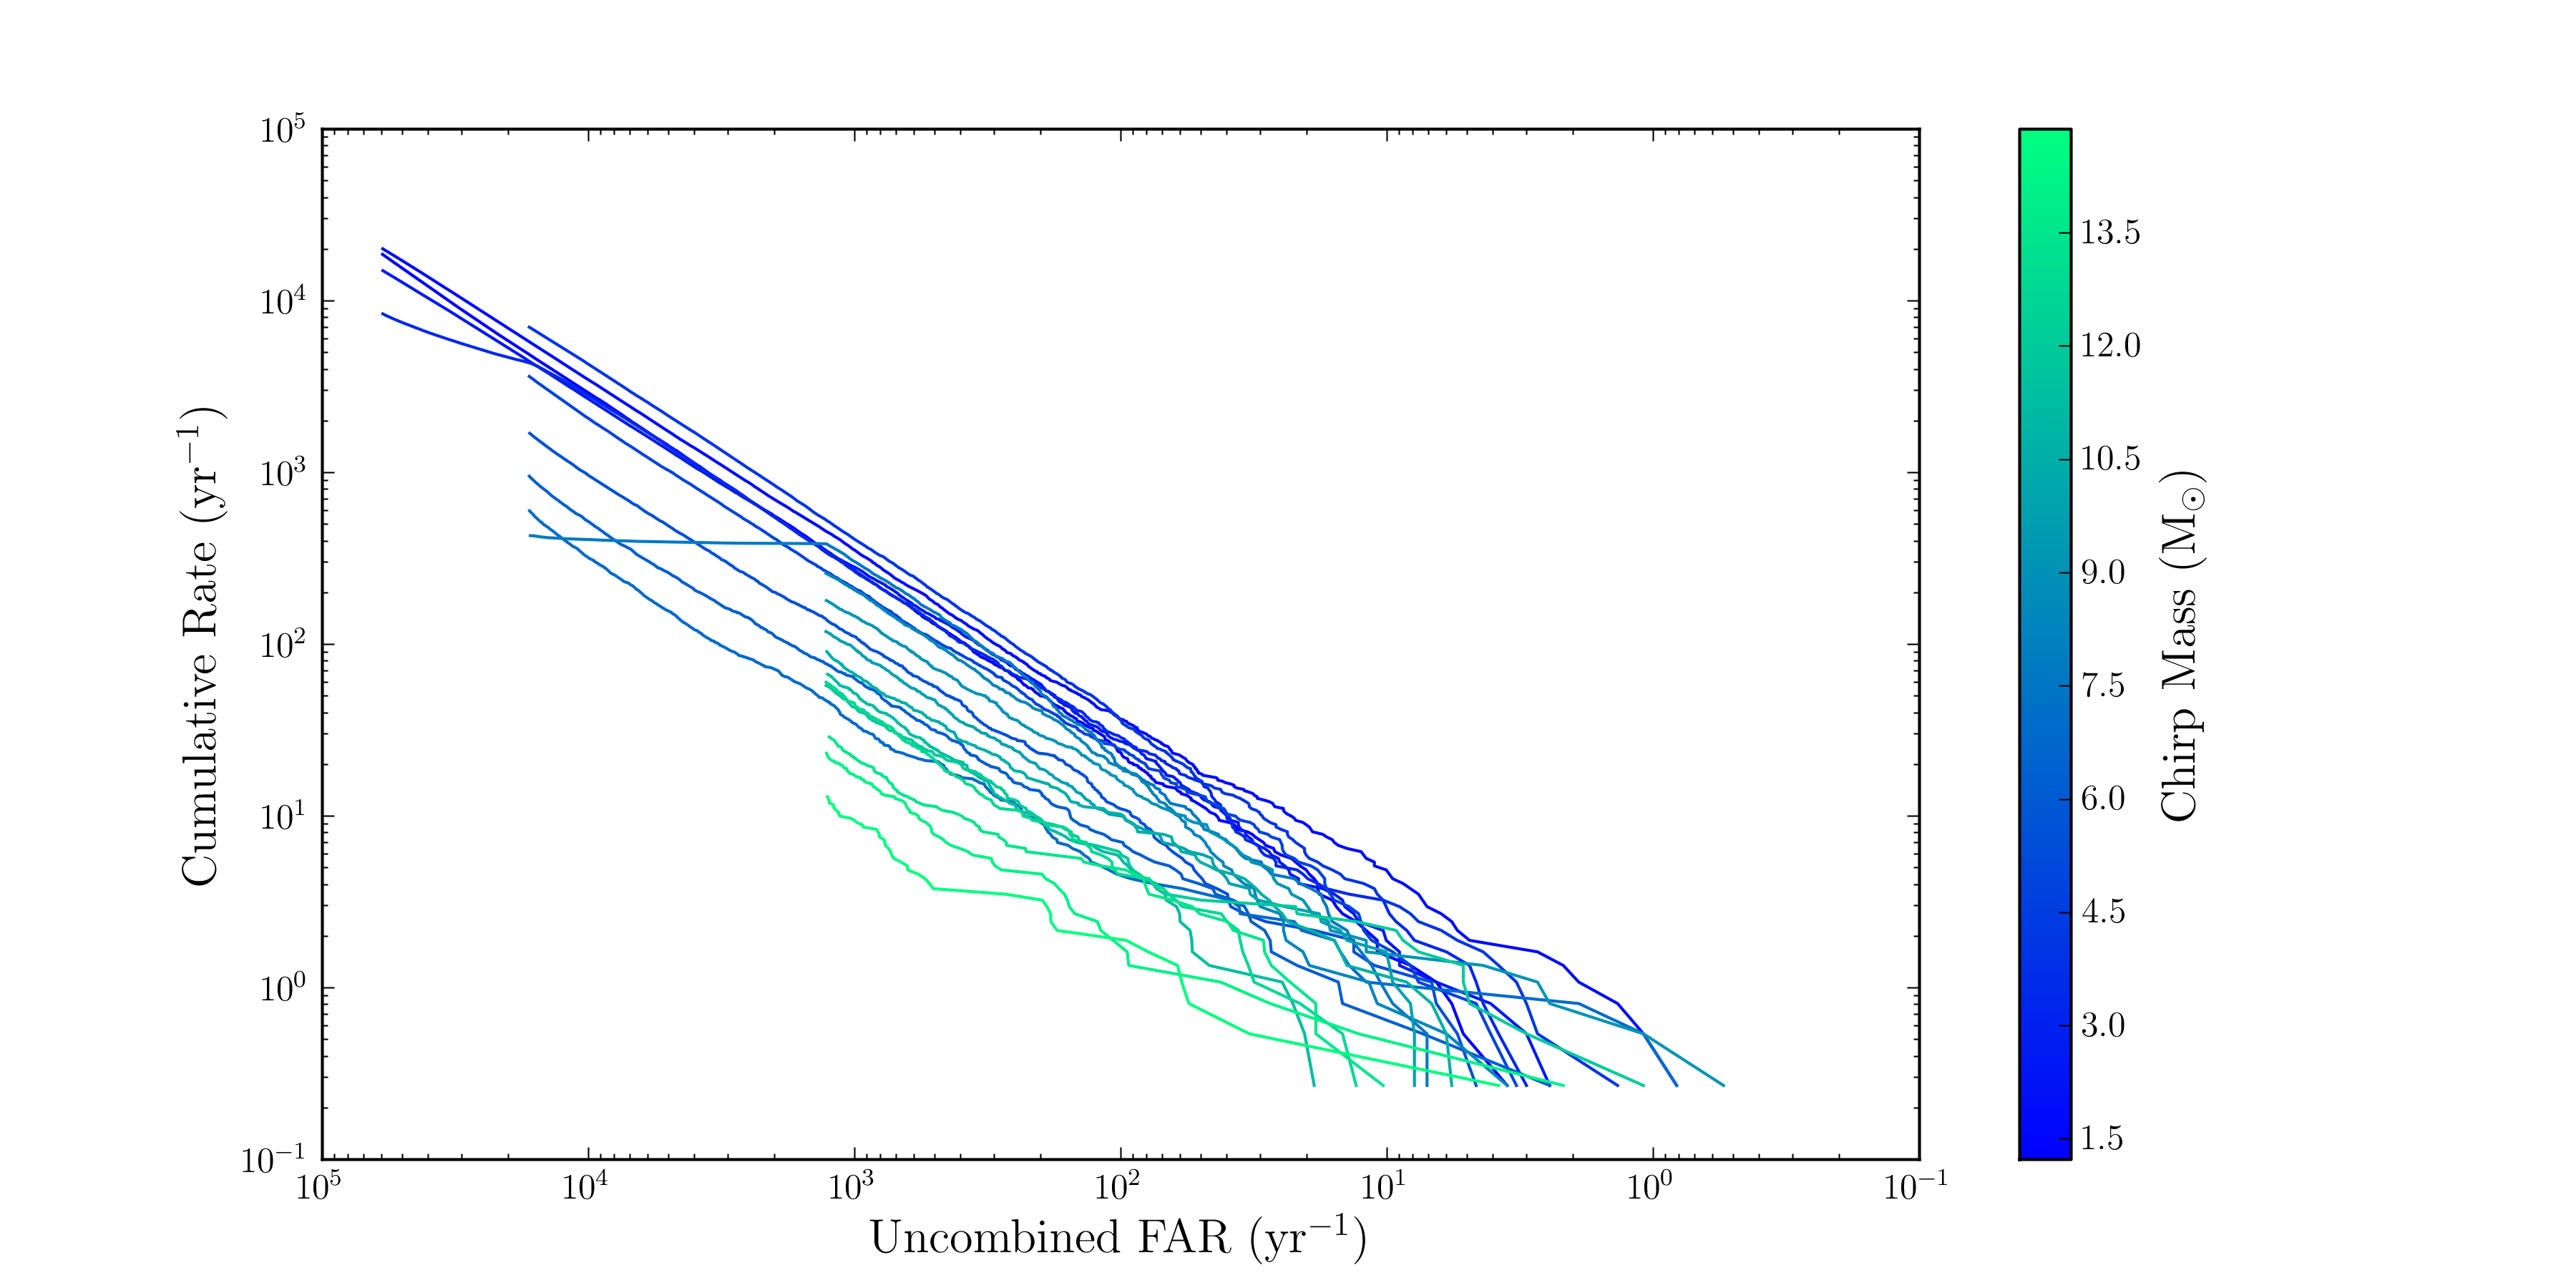
\includegraphics[width=6.5in]{figures/H1L1_H1L1-plotNdensity_cumnum_false_alarm_rate_vs_mchirp.png}}
\subfigure[Uncombined FAR v. Chirp Mass. Colored lines show lines of constant cumulative rates across the chirp-mass bins. Dashed lines show the bin boundaries used.]{\label{fig:ufar_v_mchirp-b}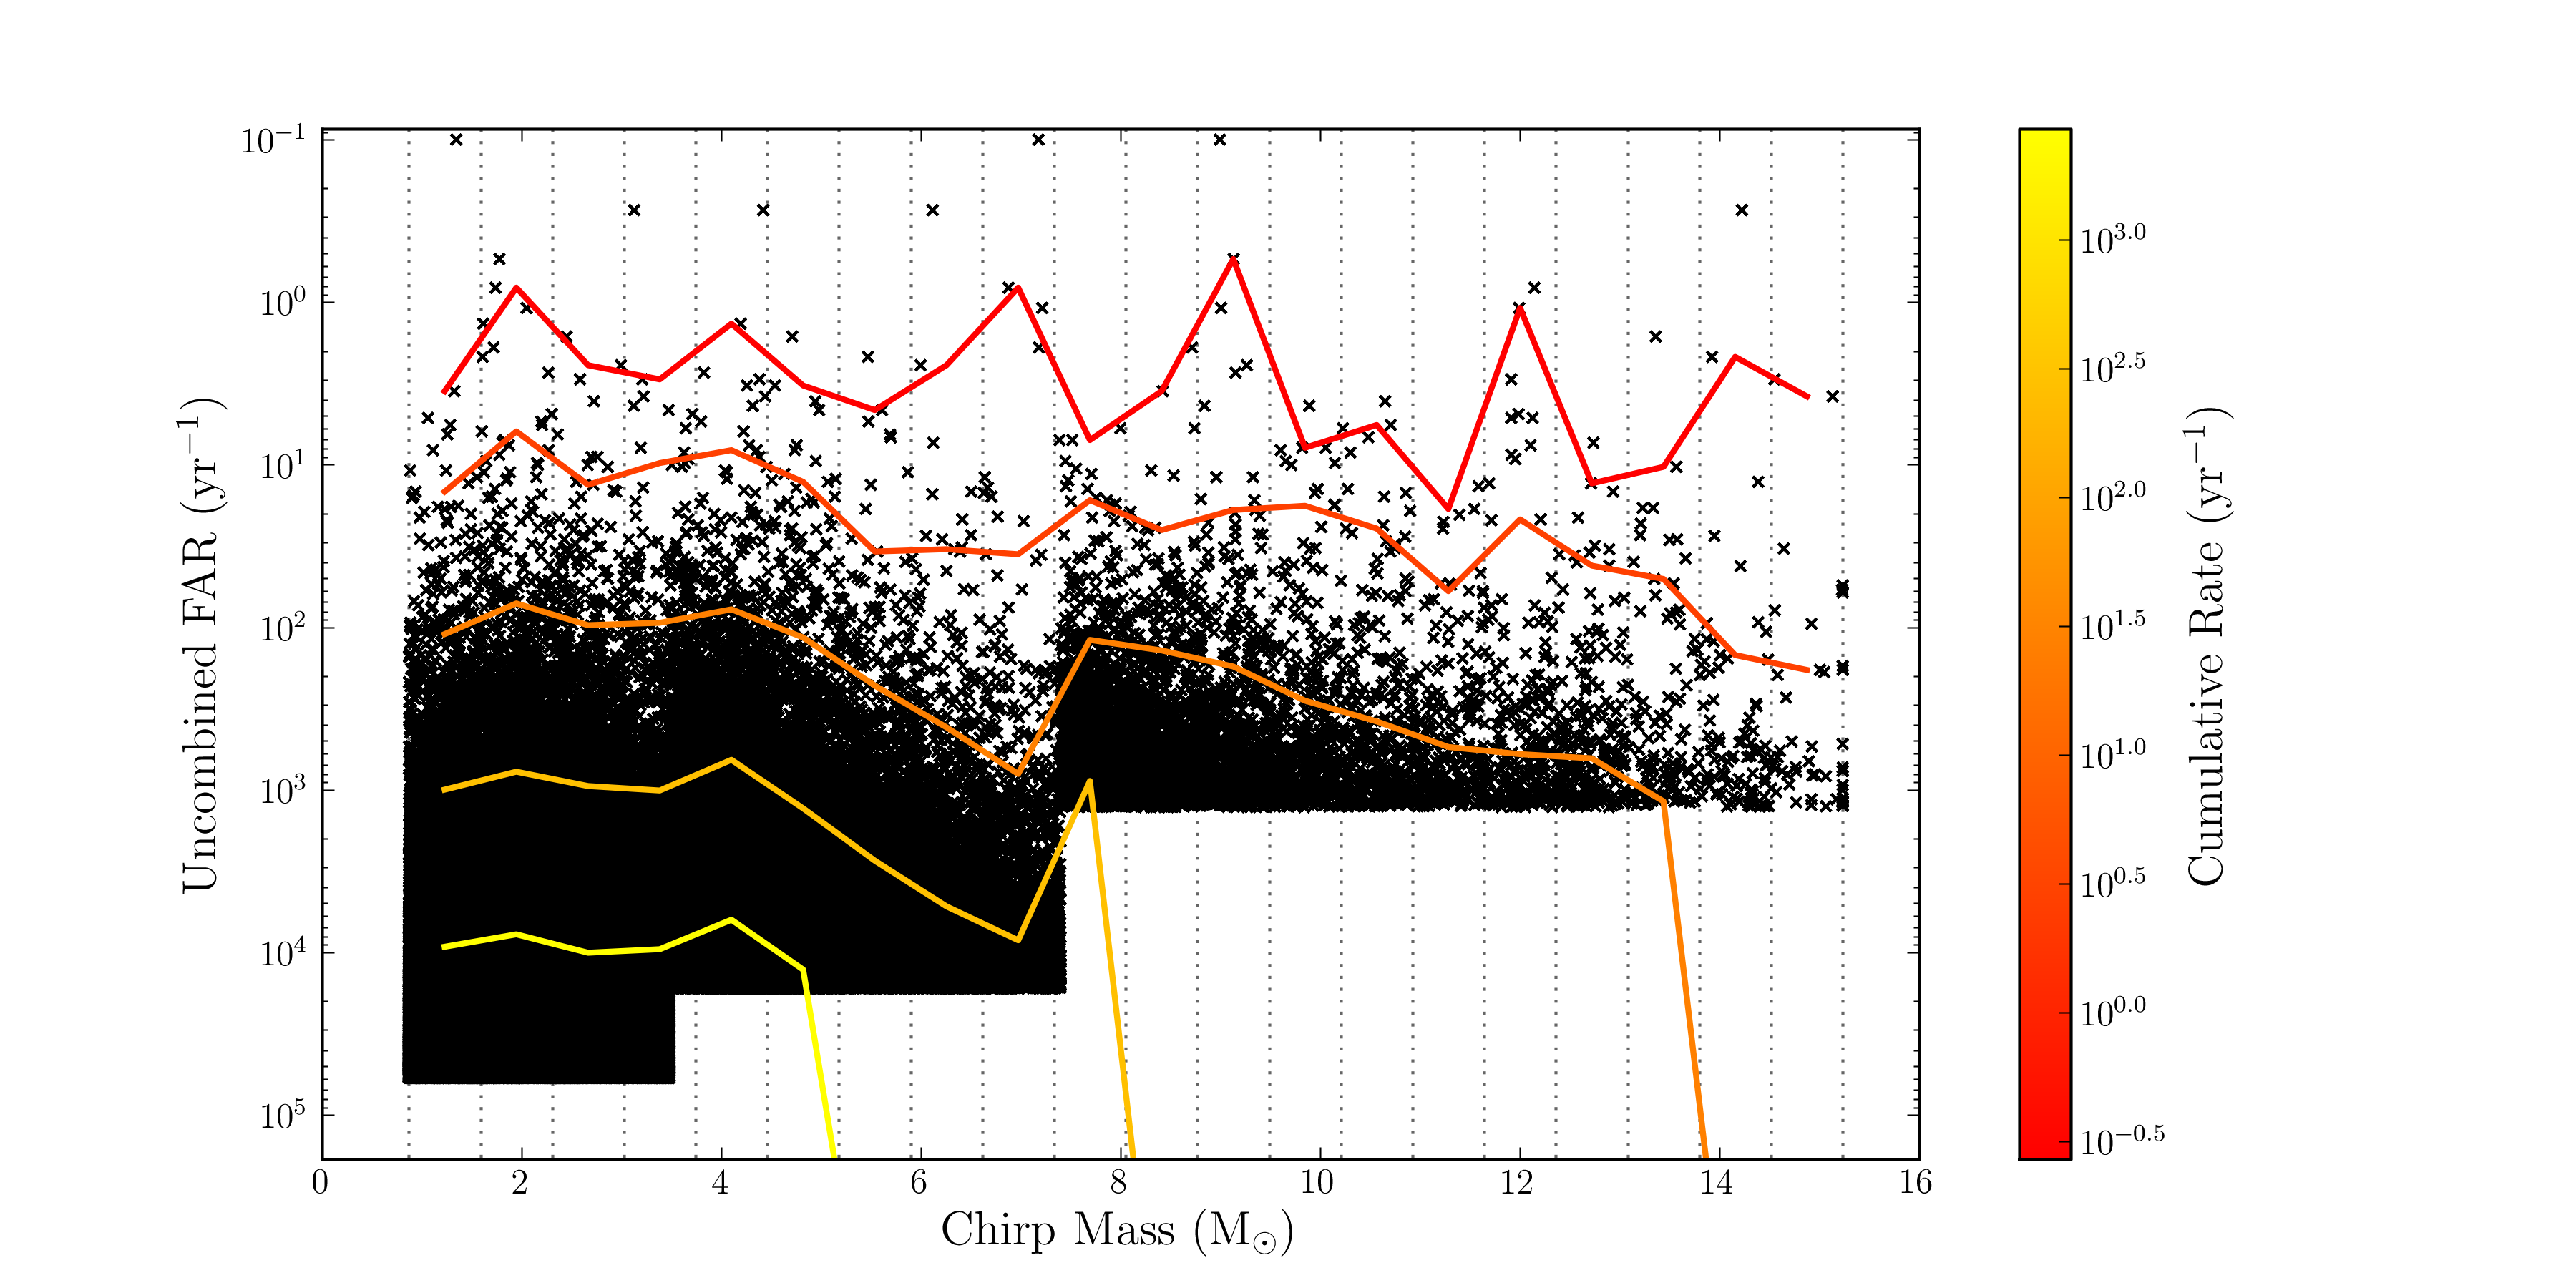
\includegraphics[width=6.5in]{figures/H1L1_H1L1-plotNdensity_false_alarm_rate_vs_mchirp.png}}
\end{center}
\caption{The rates of slide coincidences in various chirp-mass bins as a function of Uncombined \ac{FAR}. The data used is the same as that in Figure \ref{fig:newsnr_v_mchirp}. The bin boundaries used to compute the Uncombined \acp{FAR} are visible in the steps in seen in (b). The Uncombined \acp{FAR} were computed using \texttt{ligolw\_cbc\_cfar} using the same bins as used in the S5 and S6 searches (see Chapter \ref{ihope_pipeline} for details). The cumulative rates are computed by counting the number of triggers with an Uncombined \ac{FAR} $<$ each trigger within each bin. As a result the Uncombined \ac{FAR} axes are inverted. Also note that the Uncombined \ac{FAR} axes are plotted on a log scale.}
\label{fig:ufar_v_mchirp}
\end{figure}

\section{Alternate Method to Compute Combined FARs}
\label{sec:alternate_cfar_method}

There is an alternate, but equivalent, method to computing combined \acp{FAR} that does not require computing uncombined \acp{FAR} for all of the background triggers. We describe it here as it was used in the \ac{S5} search.

We begin by re-writing equation \ref{eqn:cfar_1} as an explicit sum over the number of triggers in each bin:

\begin{equation}
\label{eqn:cfar_2}
\overline{\cfar}( \far^\dagger ) = \frac{1}{\Tb} \sum_{p=1}^{N_{\mathrm{bins}}} \int_{0}^{\far^\dagger \Tb} \widehat{n}_p( \far' ) \d \far'
\end{equation}
Here, $\widehat{n}_p( \far' )$ is the measured number of triggers in $p\th$ bin with an uncombined \ac{FAR} equal to $\far'$. We expect to get roughly one trigger in each bin with a given $\far$. For example, we expect to get one trigger in each bin with a \ac{FAR} of 0, one with a \ac{FAR} of $1/\Tb$, etc. There can be some excursions from this rule; for instance, as described above, it is possible to get more than one trigger with a 0 \ac{FAR} in a single bin if one slide has more than one trigger that is louder than all triggers is all of the slides. However, if all of the slides are of roughly equal duration, then the distribution of triggers in each slide will be about the same. Thus, $\widehat{n}_p(\far') \approx 1$ for all bins and all \acp{FAR}, and equation \ref{eqn:cfar_2} becomes:

\begin{eqnarray}
\label{eqn:cfar_3}
\overline{\cfar}( \far^\dagger ) & \approx & \frac{1}{\Tb} \sum_{p=1}^{N_{\mathrm{bins}}} \int_{0}^{\far^\dagger \Tb} \d \far' \nonumber \\
 & = & N_{\mathrm{bins}} \far^\dagger
\end{eqnarray}

Again, for this to be true, the number of triggers in each bin must be about the same. As can be seen in Figure \ref{fig:ufar_v_mchirp-b} this is a valid assumption for low \acp{FAR} (the top part of the graph). However, at high \acp{FAR} (the low part of the graph), we run out of triggers in the higher mass bins. For example, consider what the combined \ac{FAR} of a trigger with $\far^\dagger = 10^4 \yr^{-1}$ would be. We can imagine drawing a horizontal line on Figure \ref{fig:ufar_v_mchirp} at $10^{-4} \yr^{-1}$ and adding up all the triggers that lie above that line. The contribution from the first two bins would be $2\far^\dagger$. However, in the third bin, the background has ``run out" at this point, so that:
\begin{equation}
\widehat{n}_3( \far' ) = \left\{ \begin{array}{l l}
    0 & \quad \mbox{if $\far' > \max(\widehat{\far}_3)$} \\
    1 & \quad \mbox{otherwise}\\ \end{array} \right.
\end{equation}
$\max(\widehat{\far}_3)$ is the largest measurable \ac{FAR} in the third bin; it is simply all the background triggers in the third bin divided by $\Tb$. Thus equation \ref{eqn:cfar_2} becomes:

\begin{eqnarray}
\label{eqn:cfar_4}
\overline{\cfar}(\far^\dagger \approx 10^{4}\yr^{-1}) & \approx & \frac{1}{\Tb} \left( 2 \int_{0}^{\far^\dagger \Tb} \d \far' + \int_{0}^{\max(\widehat{\far}_3) \Tb} \d \far' \right) \nonumber \\
 & = & 2 \far^\dagger + \max(\widehat{N}_3)/\Tb
\end{eqnarray}
where $\max(\widehat{N}_3)$ is the number of background triggers in the third bin. Likewise, if we were to measure a combined \ac{FAR} for an uncombined \ac{FAR} at $\far^\dagger = 3 \times 10^{4}$, the second bin will have run out; giving:
\begin{eqnarray}
\overline{\cfar}(\far^\dagger = 3\times 10^{4}\yr^{-1}) \approx \far^\dagger + \max(\widehat{N}_2)/\Tb + \max(\widehat{N}_3)/\Tb
\end{eqnarray}
Generalizing, we have:

\begin{equation}
\label{eqn:cfar_alt}
\overline{\cfar}(\far^\dagger) \approx N_{\mathrm{bins}}' \far^\dagger + \frac{1}{\Tb} \sum_{p=1}^{N_{\mathrm{bins}}''} \max(\widehat{N}_p)
\end{equation}
where $N_{\mathrm{bins}}'$ is the number of active bins at $\far^\dagger$, $N_{\mathrm{bins}}''$ is the number of bins that have run out, and $\max(\widehat{N}_p)$ is the total number of triggers in the $p\th$ bin. 

\section{Algorithm for Computing False Alarm Rates}
\label{sec:far_slide_algorithm}
We have arrived at an algorithm to compute false alarm rates for coincident triggers produced in a \ac{CBC} search. It is:

\begin{enumerate}
\item{Perform several time slides by adding offsets to each detector and look for coincidences across the slid detectors. The offsets should be large enough to ensure that each slide is roughly independent (i.e., at least as large as twice the time-axis of the coincidence window; larger if a single event can cause multiple triggers across several seconds).}
\item{Bin the triggers by their coincidence type and time, and, if necessary, by template parameters.}
\item{Compute an uncombined \ac{FAR} ($\overline{\far}$) for every zero-lag trigger in each bin by counting the number of slide, or background, triggers with a combined New \ac{SNR} ($\rho$) greater-than-or-equal-to the combined New \ac{SNR} of the given trigger.}
\item{Compute a final, combined \ac{FAR} ($\overline{\cfar}$) across all of the bins by either of the following methods:
    \begin{itemize}
    \item{Measure an uncombined \ac{FAR} for every background trigger by counting the number of triggers in every other slide that have a combined New \ac{SNR} that is greater-than-or-equal-to the combined New \ac{SNR} of the given trigger. Next compute a combined \ac{FAR} for the zero-lag triggers by counting the number of background triggers across all bins that have an uncombined \ac{FAR} that is less-than the given trigger.}
    \item{Use equation \ref{eqn:cfar_alt} to compute the combined \ac{FAR} directly, without computing the uncombined \acp{FAR} of the background triggers.}
    \end{itemize}}
\end{enumerate}
This method is valid as long as the number of \ac{GW}/\ac{GW} and \ac{GW}/noise coincidences in the slides are small compared to the number of noise/noise coincidences, so that equation \ref{eqn:valid_slide_condition} is valid.

\end{document}




\end{document}
